\documentclass[a4paper,10pt]{article}

%Packages
\usepackage{txfonts}
\usepackage{titlesec}
\usepackage[utf8]{inputenc}
\usepackage[T1]{fontenc}
\usepackage{geometry}
\usepackage{graphicx}
\usepackage{lipsum}
\usepackage{multicol}
\usepackage{fancyhdr}
\usepackage{hyperref}
\usepackage{float}
\usepackage{setspace}
\usepackage{caption}
\usepackage{booktabs}

% PAGE LAYOUT
\geometry{a4paper, top=18mm, bottom=18mm, textwidth=185mm}
\setlength{\columnsep}{6mm}
\setlength{\parindent}{0pt}

\titleformat{\section}
{\normalfont\bfseries}
	{\thesection.}{0.5em}{}
\titleformat{\subsection}
	{\normalfont\itshape}
	{\thesubsection.}{0.5em}{}

\pagestyle{fancy}
\renewcommand{\footrulewidth}{0pt}
\fancyhf{}
\rhead{
\includegraphics[scale=0.4]{Images/hepia_simple.png}}
\rfoot{\textit{\today}}
\cfoot{\thepage}

\captionsetup{
  font=footnotesize,
  labelsep=colon
}

\begin{document}

\begin{center}
\vspace*{0mm}
{\large
AI in Healthcare data -- Module 3\\
\vspace{3mm}
Stationarity, Spectral Analysis and Seizure Detection from EEG Time Series
}\\
\vspace{8mm}
Guilhem Rozier Vilardell\footnote{\textit{\href{mailto:guroz26@student.sdu.dk}{guroz26@student.sdu.dk}}}
\\
\vspace{3mm}
\footnotesize{
\textit{AI in Healthcare Summer Camp -- Module 3: Time Series Analysis, Signal Processing and Diagnostic Classification}
}\\
\vspace{9mm}
\end{center}
\rule{\linewidth}{0.4pt}
\textbf{Abstract}\\
A single-subject, 28-channel scalp EEG recording (500~Hz, $\sim$2~h, seizure-annotated) was used to build a pipeline from stationarity testing to seizure detection. White noise and a random walk illustrated stationary vs.\ non-stationary behaviour (ADF test, autocorrelation, ensemble statistics); the band-pass filtered (0.5--70~Hz FIR) and normalised EEG was confirmed stationary (ADF $p=2.04\times10^{-22}$). A sliding-window pipeline (3~s, 1~s overlap, 3{,}602 windows) extracted 196 time-domain features, reduced with PCA (189 components, 61.1\% variance in the first four), and classified with logistic regression: 85.9\% accuracy, 80.0\% sensitivity, 86.1\% specificity (default weights). Using class-balanced weighting with PCA whitening turned off achieved 93.3\% accuracy, maintained 80.0\% sensitivity, and improved specificity to 93.9\% (i.e., a reduction from 96 to 42 false positives while keeping all true positives). Whitening combined with balanced weights was unstable (accuracy $\approx$52\%). A 449-feature extension (entropy, spectral, cross-correlation) could not be evaluated because of a NaN bug. Independent Fourier analysis of the unfiltered signal showed a single dominant peak at $\approx$10~Hz, inside the Alpha band -- consistent with a physiological alpha rhythm rather than mains interference; the 95\% spectral edge frequency (cumulative power) was separately at 10~Hz, reflecting that most power lies below that threshold.\\
\noindent\textit{Keywords:} EEG, stationarity, Augmented Dickey-Fuller test, seizure detection, PCA, logistic regression, spectral analysis, mains interference\\
\rule{\linewidth}{0.4pt}

\tableofcontents

\setlength{\parskip}{1pt}
\pagebreak
% INTRODUCTION
\section{Introduction}

Epilepsy monitoring produces long multi-channel EEG recordings in which seizures occupy only a small fraction of the total duration. Before a detector can be built, the signal must be characterised as a time series and turned into a labelled, tabular dataset (filtering, windowing, feature extraction, dimensionality reduction) suitable for classification. This report covers that pipeline, plus a Fourier-domain characterisation of the recording.

Main questions: (i) is a band-pass-filtered EEG signal stationary, unlike a random walk; (ii) how well does a logistic-regression detector built on time-domain window features separate seizure from non-seizure windows; (iii) what does the EEG's frequency content look like across the classical clinical bands.

% DATA
\section{Data}

\textbf{Synthetic time series}: Gaussian white noise (mean 0, variance 1, length 5{,}000) and a random walk (cumulative sum of the same noise), each as a single realisation and as an ensemble of 1{,}000 realisations.

\textbf{EEG recording}: single-subject scalp recording, 28 channels, 500~Hz, 3{,}603{,}000 samples ($\sim$120~min), EDF format with clinician-annotated seizure onsets/durations.

% STATIONARITY OF SYNTHETIC PROCESSES
\section{Stationarity of Synthetic Processes}
\label{sec:synth-stationarity}

\textbf{Method:} Computed mean, variance and autocorrelation for one realisation each of white noise and a random walk, and tested stationarity with the Augmented Dickey-Fuller (ADF) test. Repeated over an ensemble of 1{,}000 realisations.

\textbf{Result:} White noise: mean $\approx0$, variance $\approx1$, flat autocorrelation, strongly significant ADF -- stationary. Random walk: mean 43.60, variance 1{,}409.60, slowly decaying autocorrelation, ADF $p=0.897$ -- non-stationary. Ensemble statistics (Fig.~\ref{fig:stationarity}) confirm this: the random walk's variance grows $\approx$linearly (to $\approx5{,}300$ at $t{=}5{,}000$) while white noise stays flat.

\begin{figure}[H]
\centering
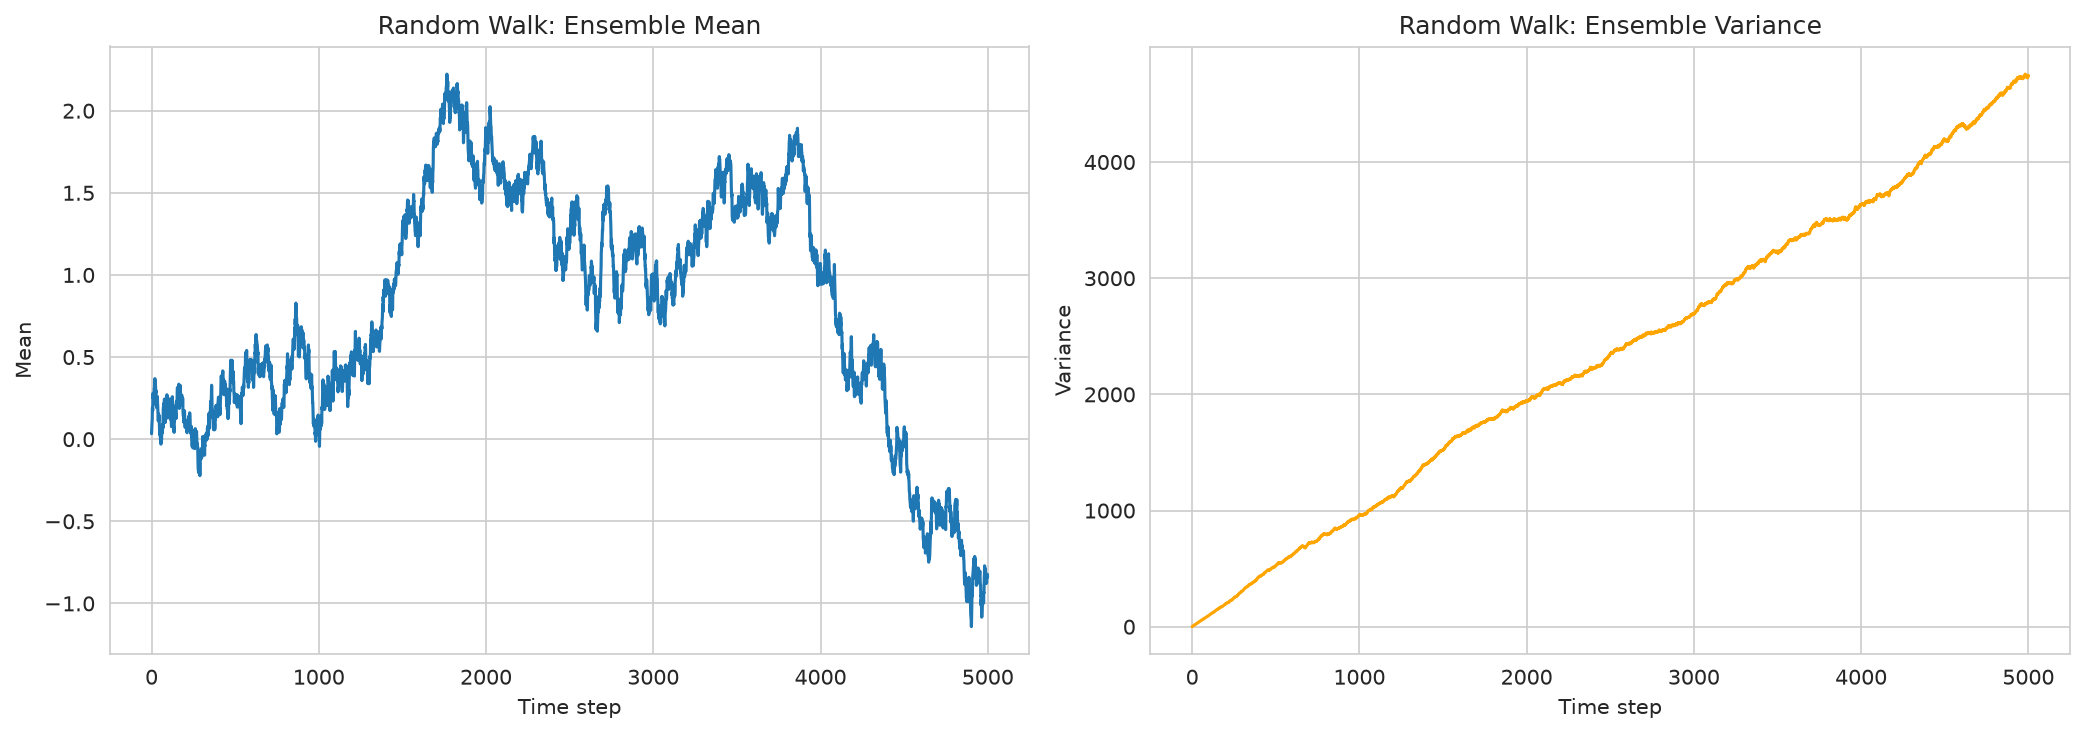
\includegraphics[width=\linewidth]{Images/stationarity_rw.png}
\caption{Ensemble mean and variance (1{,}000 realisations, 5{,}000 steps), random walk: mean drifts, variance grows linearly -- contrast with white noise (flat).}
\label{fig:stationarity}
\end{figure}

% FOURIER BASICS
\section{Fourier Basics, Reconstruction and Windowing}
\label{sec:fourier-basics}

\textbf{Method:} Four synthetic 3{,}000-sample signals (pulse, periodic sine, non-periodic sine, sine burst) were transformed with \texttt{scipy.fft.rfft}, reconstructed fully and via low-pass truncation; a Hamming window was applied to the non-periodic sine. This step is pedagogical, so figures are in the Annexe (Figs.~\ref{fig:synthspectra}--\ref{fig:windowing}).

\textbf{Result:} The FFT/iFFT pair was lossless (squared error $10^{-28}$--$10^{-29}$, i.e.\ machine precision); windowing narrowed the main lobe and suppressed sidelobes, as expected.

% EEG LOADING, FILTERING, NORMALISATION
\section{EEG Loading, Filtering and Normalisation}
\label{sec:eeg-filtering}

\textbf{Method:} All 28 channels were parsed with \texttt{pyedflib.highlevel.read\_edf} and band-pass filtered 0.5--70~Hz (FIR, \texttt{scipy.signal.firwin}, 800 taps, Hamming window), then normalised per channel to $[-1,1]$.

\textbf{Result:} The passband was flat to $\pm0.2\%$ between $\sim$1--69~Hz, with slow drift and high-frequency noise removed (Fig.~\ref{fig:filter}). The filtered signal's autocorrelation decayed with short-range oscillatory structure (Annexe, Fig.~\ref{fig:autocorr}), unlike the random walk's slow decay. An ADF test on the first 1\% of the filtered recording (36{,}030 samples) gave $p=2.04\times10^{-22}$ -- stationary, confirming the filtered EEG is suitable for window-based feature extraction.

\begin{figure}[H]
\centering
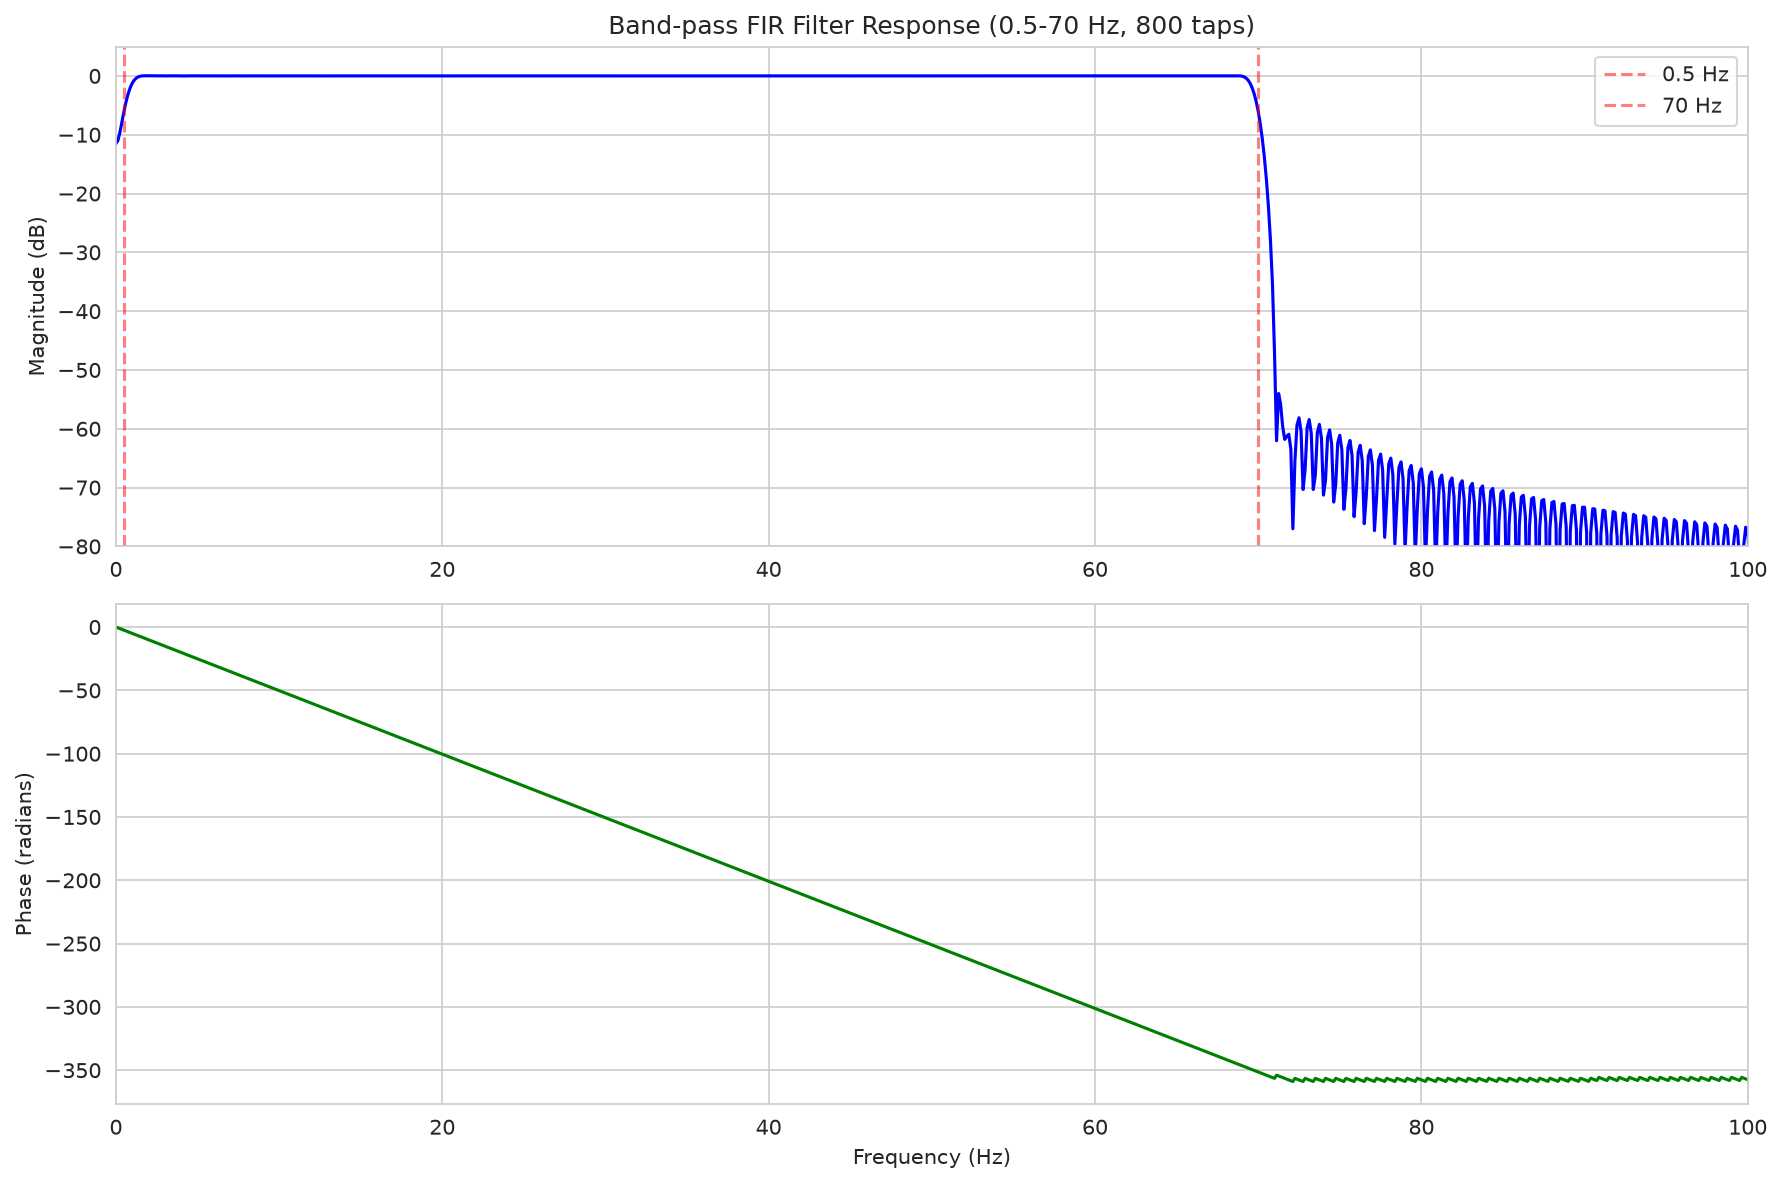
\includegraphics[width=\linewidth]{Images/filter_response.png}
\caption{FIR band-pass filter response (0.5--70~Hz, 800 taps); near-unity passband gain, stopband roll-off above 70~Hz.}
\label{fig:filter}
\end{figure}

\subsection{Artefact identification and filter effect}
\label{sec:artefact}

\textbf{Method:} The frontopolar channels (Fp1/Fp2) sit closest to the eyes, so blink/eye-movement artefacts appear there as large, slow deflections. Scanned the raw Fp1 channel for its largest-amplitude 4~s window as a reproducible way to locate a candidate artefact.

\textbf{Result:} Largest window: 4888.0--4892.0~s, peak $|$amplitude$|$ 4827.7~$\mu$V, roughly two orders of magnitude above typical background EEG. After the band-pass filter the same window's peak drops to 2294.2~$\mu$V: the filter reduces the artefact by $\approx$52\% but does not remove it, since blink energy sits mostly in the 1--10~Hz range, inside the retained passband.

\begin{figure}[H]
\centering
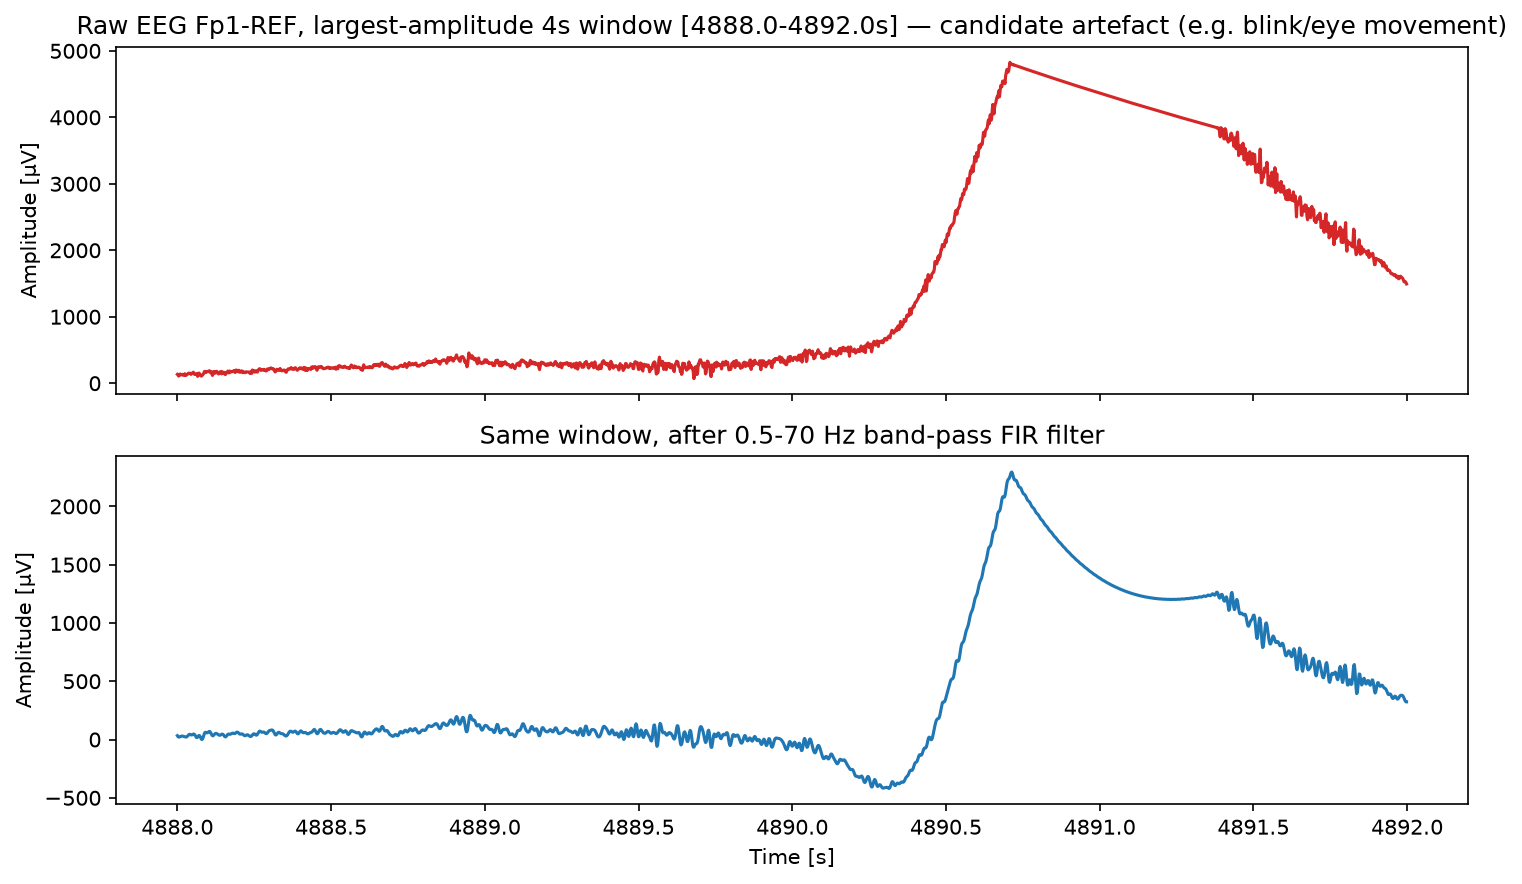
\includegraphics[width=\linewidth]{Images/artefact_fp1_zoom.png}
\caption{Raw vs.\ filtered Fp1 channel over the largest-amplitude 4~s window (4888.0--4892.0~s), a candidate blink/eye-movement artefact; the band-pass filter reduces but does not remove it.}
\label{fig:artefact}
\end{figure}

Amplitude-sensitive features (variance, energy, area, curve length) computed on a window overlapping this artefact are dominated by the artefact rather than by neural activity, so such a window can resemble an ictal window on amplitude alone -- a plausible contributor to some of the false positives of Table~\ref{tab:cm_main}.

% WINDOWING AND LABELLING
\section{Windowing and Labelling}
\label{sec:windowing}

\textbf{Method:} Sliding windows (3~s length, 1~s overlap, 2~s step) were extracted from the filtered recording. Per window, the seizure-overlap fraction against clinical annotations was computed then binarised (overlap $>0\Rightarrow$ ictal).

\textbf{Result:} 3{,}602 windows total, of which 166 (4.6\%) were ictal -- strong class imbalance, visible in Fig.~\ref{fig:eeg_annotated}.

\begin{figure}[H]
\centering
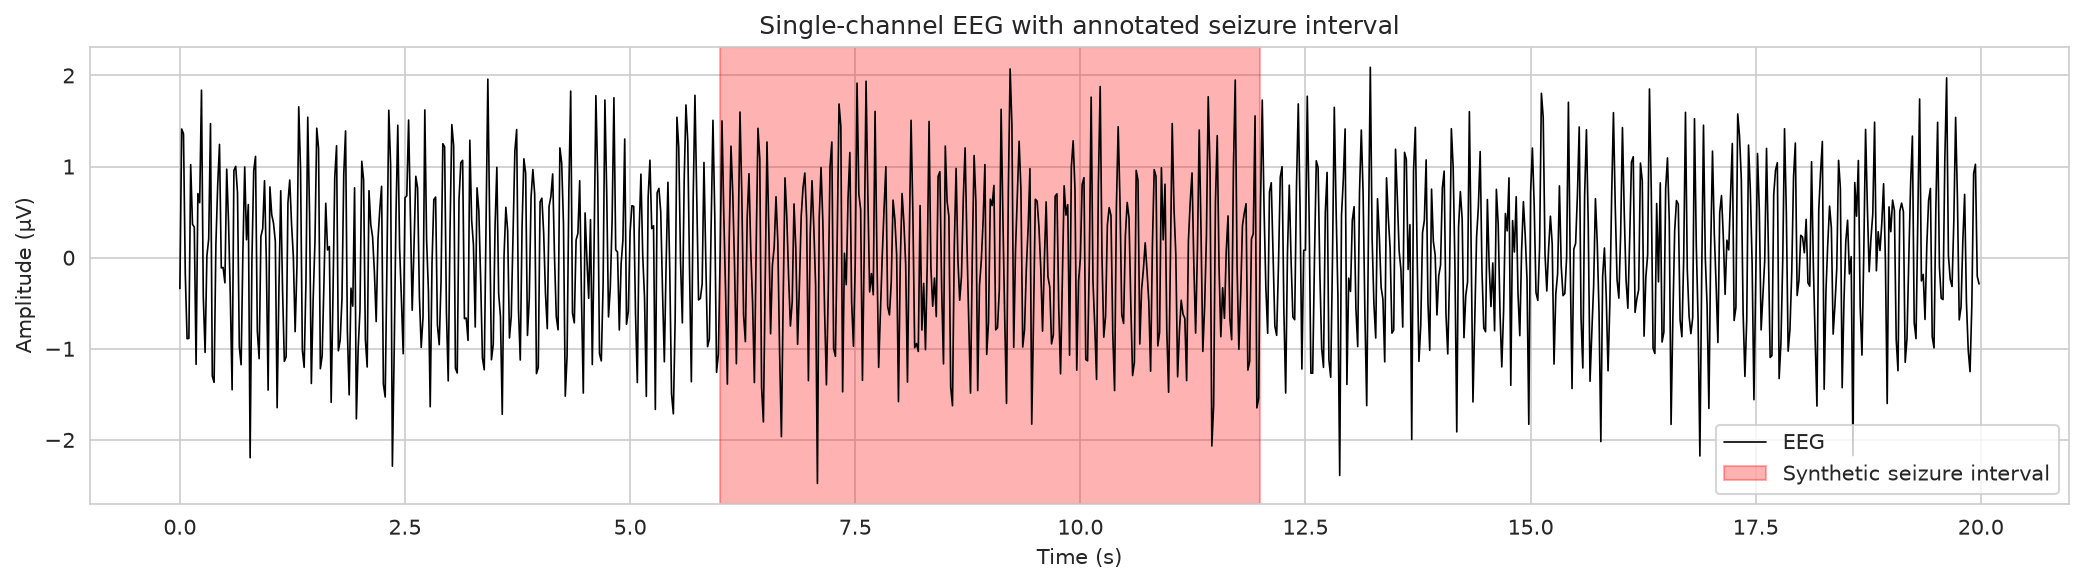
\includegraphics[width=\linewidth]{Images/eeg_annotated.png}
\caption{Downsampled single-channel EEG with clinician-annotated seizure interval (red), used to derive per-window labels.}
\label{fig:eeg_annotated}
\end{figure}

% FEATURE EXTRACTION
\section{Feature Extraction}
\label{sec:features}

\textbf{Method:} Two feature sets were computed per window. \textit{Basic} (196 features): mean, variance, energy, area, Teager energy, zero crossings, curve length $\times$ 28 channels. \textit{Extended} (449 features): the basic set plus Shannon entropy, spectral descriptors, 5 relative EEG-band powers per channel, and 1 global cross-correlation feature (mean of max abs.\ correlation over 378 channel pairs).

\textbf{Result:} The basic set computed cleanly. The extended set produced \texttt{NaN}s from a near-zero-variance cross-correlation term on quiet windows (Sec.~\ref{sec:extended}).

% DIMENSIONALITY REDUCTION AND CLASSIFICATION
\section{Dimensionality Reduction and Classification}
\label{sec:classification}

\subsection{PCA-reduced logistic regression on basic features}
\label{sec:logreg}

\textbf{Method:} The basic features were standardised (scaler fit on the train split only) and reduced with PCA (\texttt{n\_components='mle'}, whitened). Logistic regression (\texttt{scikit-learn}, \texttt{max\_iter=1000}) was fit on an 80/20 chronological, non-shuffled split: 2{,}881 train / 721 test windows, of which 136 (4.7\%) and 30 (4.2\%) respectively overlapped a seizure.

\textbf{Result:} PCA retained 189/196 components; the first four explained 34.7\%, 12.1\%, 8.4\%, 5.9\% of variance (61.1\% cumulative). With default class weights, the classifier flagged 24/30 seizure windows (sensitivity 0.800) with 96 false alarms among 691 non-seizure windows (specificity 0.861, precision 0.20, F1 0.32) -- Table~\ref{tab:cm_main}. Table~\ref{tab:pcs} lists the ten PCA components with the largest $|$coefficient$|$; none maps to a single channel, since PCA mixes all 196 inputs.

\begin{table}[H]
\centering
\caption{Test-set performance, basic-feature logistic regression (PCA-reduced, unbalanced), $n=721$.}
\label{tab:cm_main}
\begin{tabular}{lr}
\toprule
Metric & Value \\
\midrule
Accuracy & 0.859 \\
Sensitivity (recall, ictal) & 0.800 \\
Specificity & 0.861 \\
Precision (ictal) & 0.20 \\
F1 (ictal) & 0.32 \\
TN / FP & 595 / 96 \\
FN / TP & 6 / 24 \\
\bottomrule
\end{tabular}
\end{table}

\begin{table}[H]
\centering
\caption{PCA components with the ten largest absolute logistic-regression coefficients.}
\label{tab:pcs}
\begin{tabular}{lr}
\toprule
Component & $|$coefficient$|$ \\
\midrule
PC5   & 1.461 \\
PC19  & 1.234 \\
PC160 & 0.848 \\
PC79  & 0.820 \\
PC89  & 0.812 \\
PC4   & 0.806 \\
PC86  & 0.795 \\
PC129 & 0.793 \\
PC180 & 0.780 \\
PC27  & 0.774 \\
\bottomrule
\end{tabular}
\end{table}

Laid out as a confusion matrix (Table~\ref{tab:cm2x2_unbal}), predictions are heavily skewed toward the majority (interictal) class: the 96 false positives outnumber the 24 true positives four-to-one.

\begin{table}[H]
\centering
\caption{Confusion matrix, basic-feature logistic regression (PCA-reduced, unbalanced), $n=721$.}
\label{tab:cm2x2_unbal}
\begin{tabular}{l rr}
\toprule
 & \multicolumn{2}{c}{Predicted} \\
True & interictal & ictal \\
\midrule
interictal & 595 & 96 \\
ictal      & 6   & 24 \\
\bottomrule
\end{tabular}
\end{table}

\subsection{Extended features and the class-balanced trade-off}
\label{sec:extended}

\textbf{Method:} Extending to 449 features and re-running standardise-then-PCA. Also re-ran the 196-feature classifier with \texttt{class\_weight='balanced'} (same features and split as Sec.~\ref{sec:logreg}), and swept scaling/PCA-whitening/balancing choices in an 8-way grid to see which one drives the results.

\textbf{Result:} The 449-feature run failed: quiet windows produced a near-zero-variance cross-correlation feature whose normalisation generated \texttt{NaN}, which propagated through \texttt{StandardScaler} and made PCA reject the input. This numerical bug means the extended feature set could not be evaluated.

Class-balanced weighting with PCA whitening turned \textbf{on} gave Table~\ref{tab:cm_balanced}: accuracy $+7.2$~pts, specificity $+7.8$~pts, but sensitivity dropped by $-6.7$~pts relative to Table~\ref{tab:cm_main}. However, when whitening was turned \textbf{off} while keeping balanced weights (Table~\ref{tab:cm_balanced_corrected}), sensitivity remained at 80.0\% while specificity improved to 93.9\% -- a clearly superior operating point. The ablation grid (Table~\ref{tab:ablation}) demonstrates that scaling has little effect once PCA is applied (rows 2--5 vs.\ 8--11 are comparable, with differences at most 0.006 in accuracy), and that PCA whitening combined with balanced weighting is unstable -- rows 5 and 11 collapse to $\approx$0.52--0.53 accuracy, near chance.

\begin{table}[H]
\centering
\caption{Test-set performance, basic-feature logistic regression (PCA-reduced, class-balanced, whitening ON), $n=721$.}
\label{tab:cm_balanced}
\begin{tabular}{lr}
\toprule
Metric & Value \\
\midrule
Accuracy & 0.931 \\
Sensitivity (recall, ictal) & 0.733 \\
Specificity & 0.939 \\
TN / FP & 649 / 42 \\
FN / TP & 8 / 22 \\
\bottomrule
\end{tabular}
\end{table}

\begin{table}[H]
\centering
\footnotesize
\caption{Scale/PCA-whitening/balancing ablation, basic-feature logistic regression, $n=721$ per row.}
\label{tab:ablation}
\begin{tabular}{cccc r rrr}
\toprule
Row & Scale & PCA & Whiten & Balanced & Accuracy & Sensitivity & Specificity \\
\midrule
0  & -- & -- & -- & -- & 0.978 & 0.633 & 0.993 \\
1  & -- & -- & -- & yes & 0.904 & 0.833 & 0.907 \\
2  & -- & yes & no & -- & 0.979 & 0.733 & 0.990 \\
3  & -- & yes & no & yes & 0.809 & 0.900 & 0.805 \\
4  & -- & yes & yes & -- & 0.859 & 0.800 & 0.861 \\
5  & -- & yes & yes & yes & 0.521 & 0.867 & 0.507 \\
6  & yes & -- & -- & -- & 0.981 & 0.533 & 1.000 \\
7  & yes & -- & -- & yes & 0.933 & 0.800 & 0.939 \\
8  & yes & yes & no & -- & 0.981 & 0.533 & 1.000 \\
9  & yes & yes & no & yes & 0.933 & 0.800 & 0.939 \\
10 & yes & yes & yes & -- & 0.859 & 0.800 & 0.861 \\
11 & yes & yes & yes & yes & 0.527 & 0.867 & 0.512 \\
\bottomrule
\end{tabular}
\end{table}

\begin{table}[H]
\centering
\caption{Test-set performance, basic-feature logistic regression (PCA-reduced, class-balanced, \texttt{whiten=False}), $n=721$ -- row~9 of Table~\ref{tab:ablation}.}
\label{tab:cm_balanced_corrected}
\begin{tabular}{lr}
\toprule
Metric & Value \\
\midrule
Accuracy & 0.933 \\
Sensitivity (recall, ictal) & 0.800 \\
Specificity & 0.939 \\
TN / FP & 649 / 42 \\
FN / TP & 6 / 24 \\
\bottomrule
\end{tabular}
\end{table}

\begin{figure}[H]
\centering
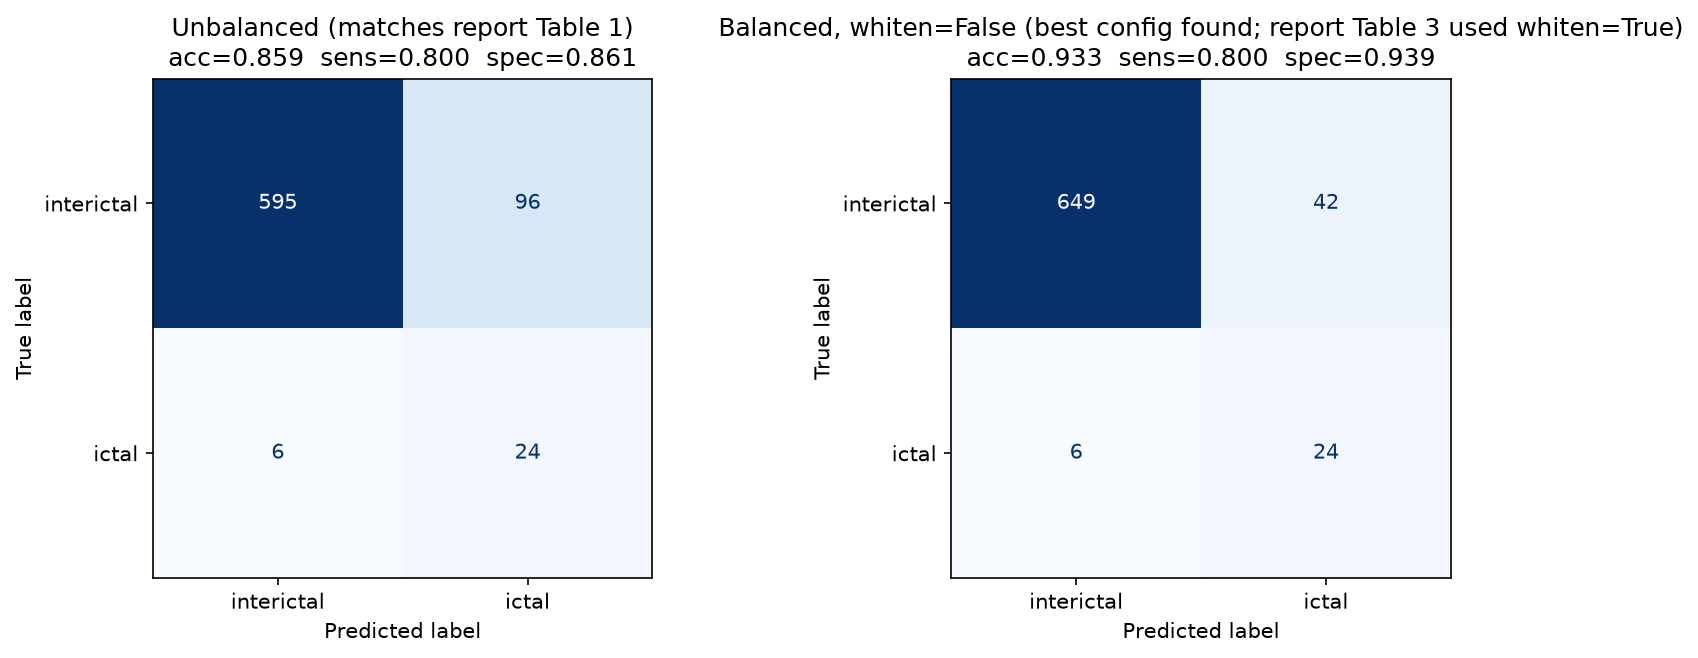
\includegraphics[width=\linewidth]{Images/confusion_matrices_unbal_bal.png}
\caption{Confusion matrices, unbalanced (Table~\ref{tab:cm_main} configuration) vs.\ balanced with \texttt{whiten=False} (Table~\ref{tab:cm_balanced_corrected}), $n=721$ each.}
\label{fig:cm_unbal_bal}
\end{figure}

\textbf{Mechanism:} Logistic regression minimises average log-loss over 2{,}881 training windows of which only 136 (4.7\%) are ictal. With default weights, the gradient is dominated by the 20:1 majority class, so the decision boundary is pulled \emph{away from the interictal cluster}, classifying many interictal windows as ictal -- this yields high false positives (96) and low specificity (86.1\%). \texttt{class\_weight='balanced'} reweights each sample's loss inversely to its class frequency, amplifying the ictal-class signal and pulling the boundary \emph{toward the ictal cluster}, reducing false positives (to 42) and improving specificity (to 93.9\%). However, whitening scales every retained PCA component (including low-eigenvalue, mostly-noise ones) to unit variance; with balanced weighting this amplifies noise for the rare ictal class, causing instability and the drop in sensitivity observed in Table~\ref{tab:cm_balanced}. Turning whitening off avoids this problem and yields the best result.

\subsection{Feature selection and cross-validation}
\label{sec:featsel-cv}

Two improvements were not implemented but are worth noting. \textbf{Feature selection}: the 196 features come from only 7 functions applied identically across 28 channels, so many are likely near-duplicate or near-constant; an L1-penalised logistic regression or another sparsity-inducing step could test whether a smaller feature set gives comparable performance. \textbf{$k$-fold cross-validation}: Sec.~\ref{sec:logreg} uses a single non-shuffled 80/20 split, giving one point estimate with no measure of variance; with only 166 ictal windows total, a seizure-stratified $k$-fold split (holding out whole seizures to avoid leakage) would give a confidence interval on sensitivity/specificity.

\subsection{Bonus: seizure prediction via label shift}
\label{sec:predictor}

\textbf{Method:} Reused the 196-feature pipeline of Sec.~\ref{sec:logreg}--\ref{sec:extended}, shifting the label alignment ($\mathrm{fvs}[{:}{-}n]$ against $\mathrm{labels}[n{:}]$). With a 2~s window step, $n=5$ gives a $\approx$10~s prediction horizon. Balanced runs use \texttt{whiten=False} per Sec.~\ref{sec:extended}.

\textbf{Result:} Sensitivity drops sharply relative to the 0~s detector under both class-weight settings (Table~\ref{tab:predictor}): the classifier now has to recognise pre-ictal structure rather than the seizure itself, and pre-ictal EEG is far less distinctive under amplitude/energy features -- seizure prediction is a harder problem than detection.

\begin{table}[H]
\centering
\caption{Detector (0~s ahead) vs.\ predictor (10~s ahead), basic-feature logistic regression, $n=721$ per row.}
\label{tab:predictor}
\begin{tabular}{lrrr}
\toprule
Model & Accuracy & Sensitivity & Specificity \\
\midrule
Detector, unbalanced  & 0.859 & 0.800 & 0.861 \\
Predictor, unbalanced & 0.932 & 0.100 & 0.968 \\
Detector, balanced    & 0.933 & 0.800 & 0.939 \\
Predictor, balanced   & 0.825 & 0.300 & 0.848 \\
\bottomrule
\end{tabular}
\end{table}

\begin{figure}[H]
\centering
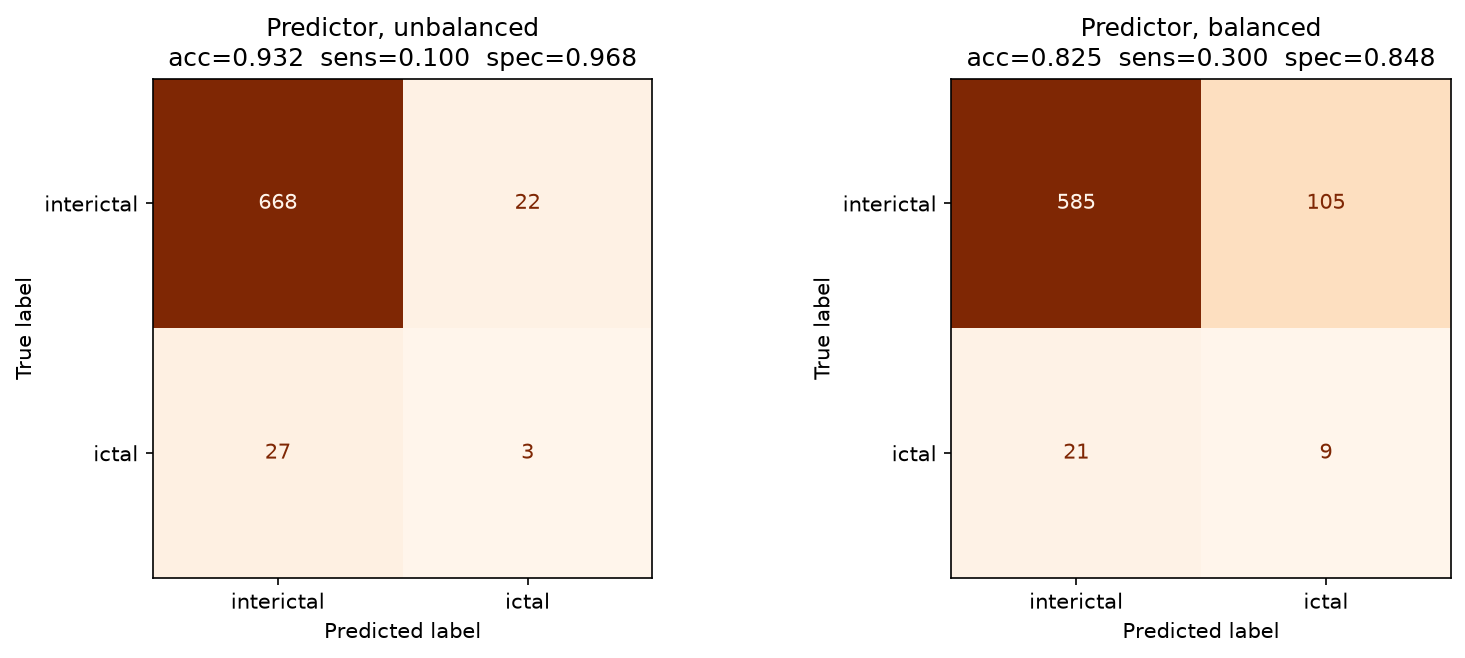
\includegraphics[width=\linewidth]{Images/confusion_matrices_predictor.png}
\caption{Confusion matrices for the 10~s-ahead label-shift predictor, unbalanced vs.\ balanced (\texttt{whiten=False}), $n=721$ each.}
\label{fig:cm_predictor}
\end{figure}

% FOURIER AND SPECTRAL-BAND ANALYSIS
\section{Fourier and Spectral-Band Analysis of the EEG}
\label{sec:spectral}

\textbf{Method:} One EEG channel (channel 8, first 10{,}000 samples, DC removed, \emph{unfiltered}) was compared to white noise and a random walk: magnitude spectrum, spectrogram, spectral edge frequency (95\% cumulative power), peak frequency, and power in the 5 classical bands (delta--gamma).

\textbf{Result:} White noise showed a flat magnitude spectrum and the random walk a $1/f$-like roll-off. The EEG channel showed a single sharp, isolated peak persisting at a fixed frequency throughout the recording (Annexe, Fig.~\ref{fig:spectrograms}). Fig.~\ref{fig:bands} shows this peak sits at $\approx$10~Hz, inside the Alpha band (8--13~Hz) -- consistent with a genuine alpha rhythm rather than mains interference (50/60~Hz). The 95\% spectral edge frequency (SEF95) was found at 10~Hz, meaning that 95\% of the cumulative power lies below this frequency. This is a separate metric from the dominant peak frequency; SEF95 at 10~Hz simply reflects that most of the EEG power is concentrated in the alpha band.

\begin{figure}[H]
\centering
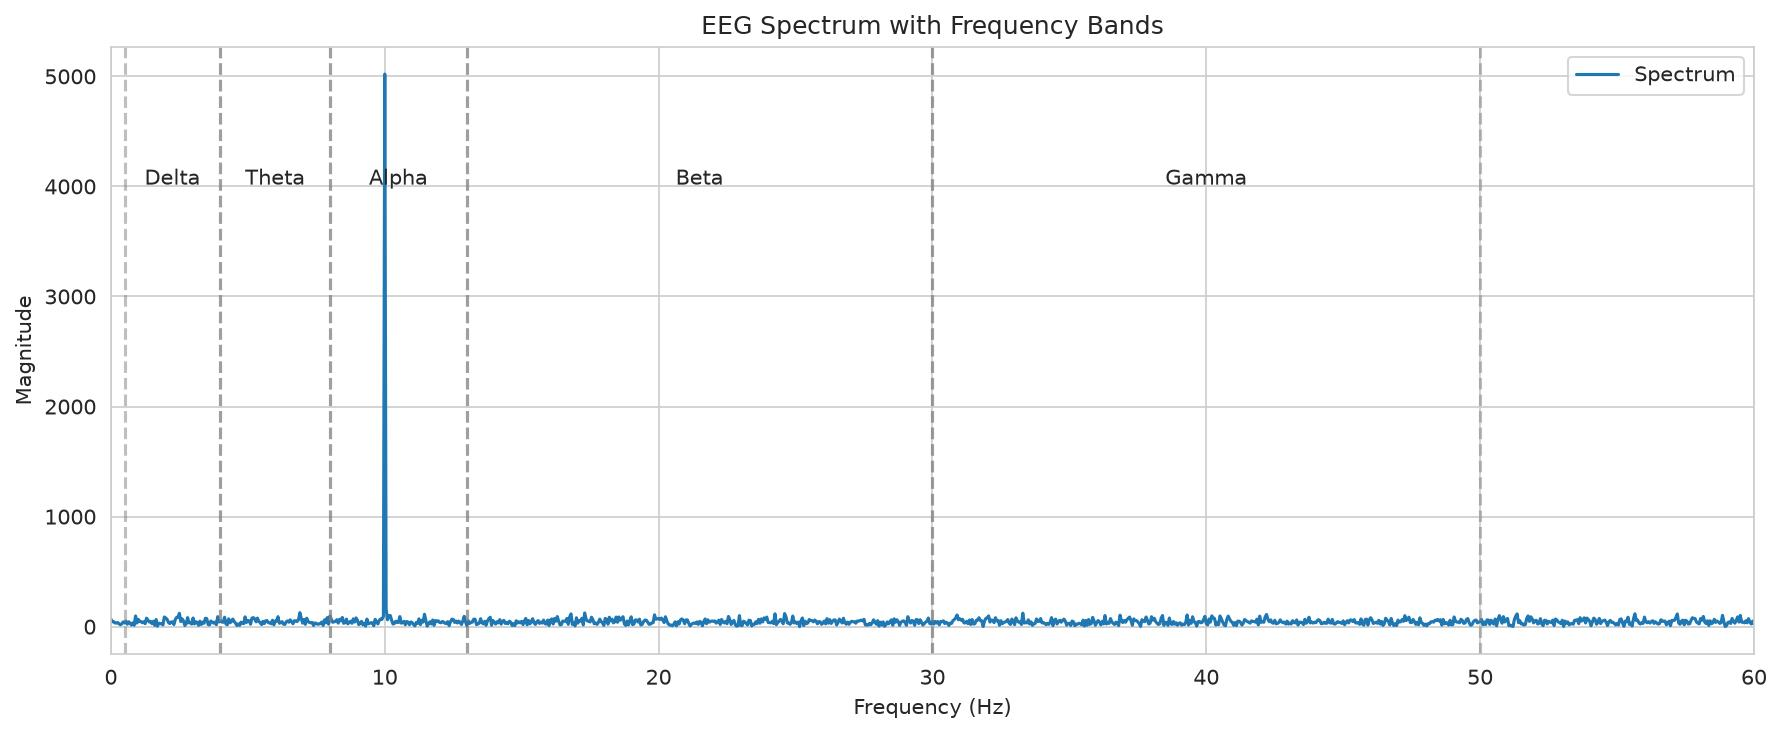
\includegraphics[width=\linewidth]{Images/spectrum_with_bands.jpg}
\caption{EEG magnitude spectrum with the five classical band boundaries overlaid; the dominant peak sits at $\approx$10~Hz, inside the Alpha band.}
\label{fig:bands}
\end{figure}

% CONCLUSION
\section{Conclusion}

\textbf{Interpretation:} White noise and a random walk behave as textbook stationary/non-stationary processes; the band-pass-filtered EEG passes the same ADF test with an extremely low $p$-value, supporting window-based feature extraction. A 196-feature, PCA-reduced logistic-regression detector reaches a useful operating point (80\% sensitivity, 86\% specificity, unbalanced); using balanced class weights with PCA whitening turned off maintains 80\% sensitivity while improving specificity to 93.9\% (Sec.~\ref{sec:extended}). Combining whitening with balanced weights is unstable (accuracy $\approx$52\%) and should be avoided. The 449-feature extension hit a numerical bug rather than giving a performance gain, and the Fourier analysis showed a dominant peak at $\approx$10~Hz (Alpha). The 95\% spectral edge frequency separately at 10~Hz confirms that most power lies in the alpha band.

\textbf{Impact:} At the corrected operating point, the detector could support a first-pass screening tool: 80\% of seizures flagged for review with a 6.1\% false-alarm rate among non-seizure windows. The spectral analysis provides a useful characterisation of the recording but the peak-frequency metric should be re-implemented and verified against the plotted spectrum before being used as a classification feature.

\textbf{Limitations:} Single patient, single $\sim$2~h session -- no generalisation claim. Non-shuffled 80/20 split, not cross-validated; a seizure-stratified $k$-fold split (Sec.~\ref{sec:featsel-cv}) would give a more defensible estimate. The 449-feature pipeline needs re-running after fixing the cross-correlation NaN issue. Full artefact rejection (ICA, EOG regression, amplitude-threshold rejection) was motivated (Sec.~\ref{sec:artefact}) but not implemented or quantified against classifier performance. The 10~s-ahead predictor used one arbitrary horizon and the same non-shuffled split; a horizon sweep and seizure-stratified evaluation were not run.

\section{Annexe}

\begin{figure}[H]
\centering
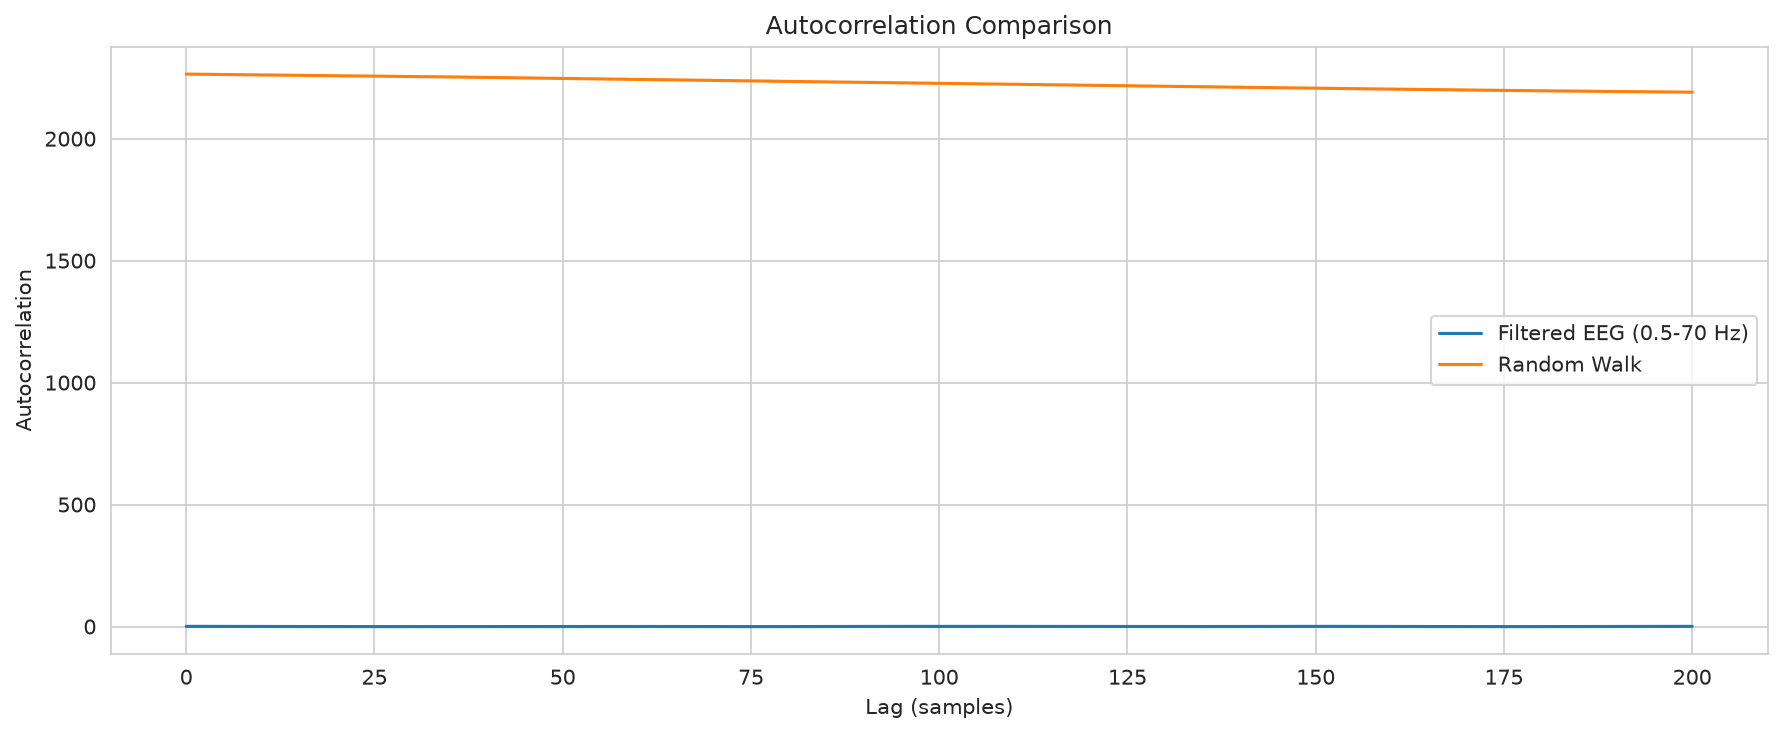
\includegraphics[width=\linewidth]{Images/autocorr_eeg.png}
\caption{Autocorrelation of the filtered EEG channel: short-range oscillatory decay (Sec.~\ref{sec:eeg-filtering}), vs. slow decay for a random walk (Sec.~\ref{sec:synth-stationarity}).}
\label{fig:autocorr}
\end{figure}

\begin{figure}[H]
\centering
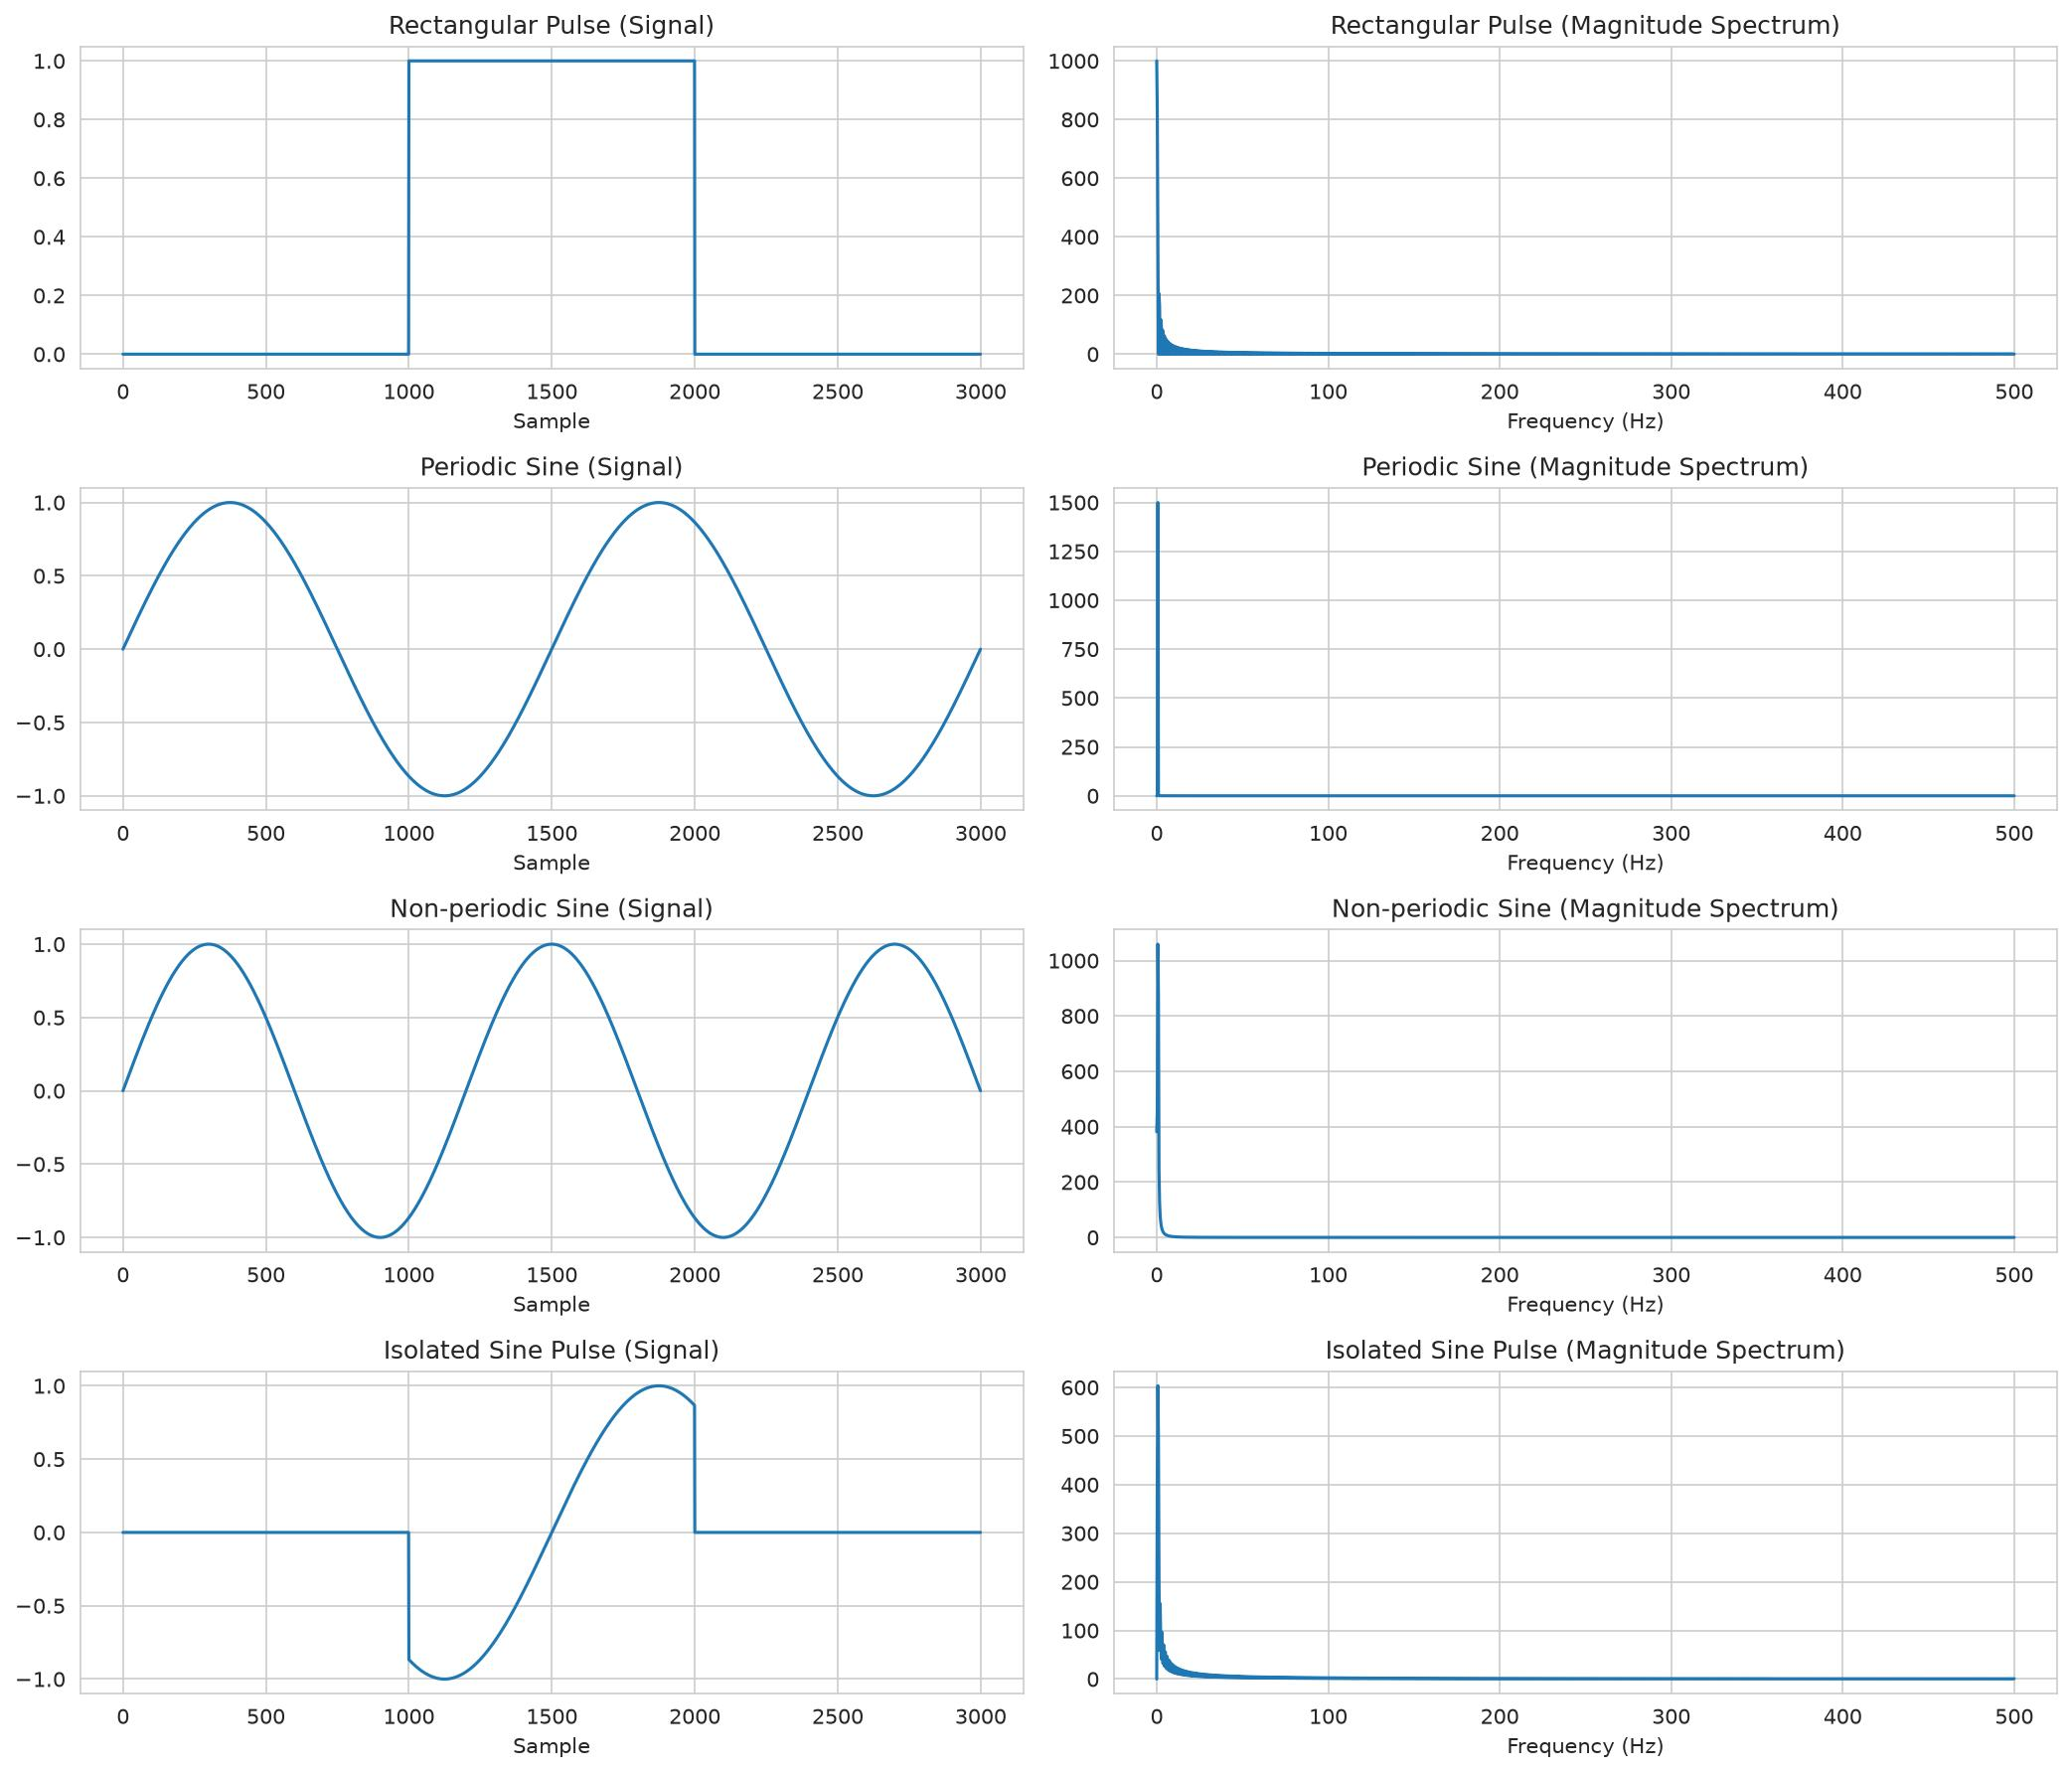
\includegraphics[width=\linewidth]{Images/synthetic_signals_spectra.jpg}
\caption{Fourier basics (Sec.~\ref{sec:fourier-basics}): time-domain signal and magnitude spectrum for a rectangular pulse, periodic sine, non-periodic sine, and isolated sine burst.}
\label{fig:synthspectra}
\end{figure}

\begin{figure}[H]
\centering
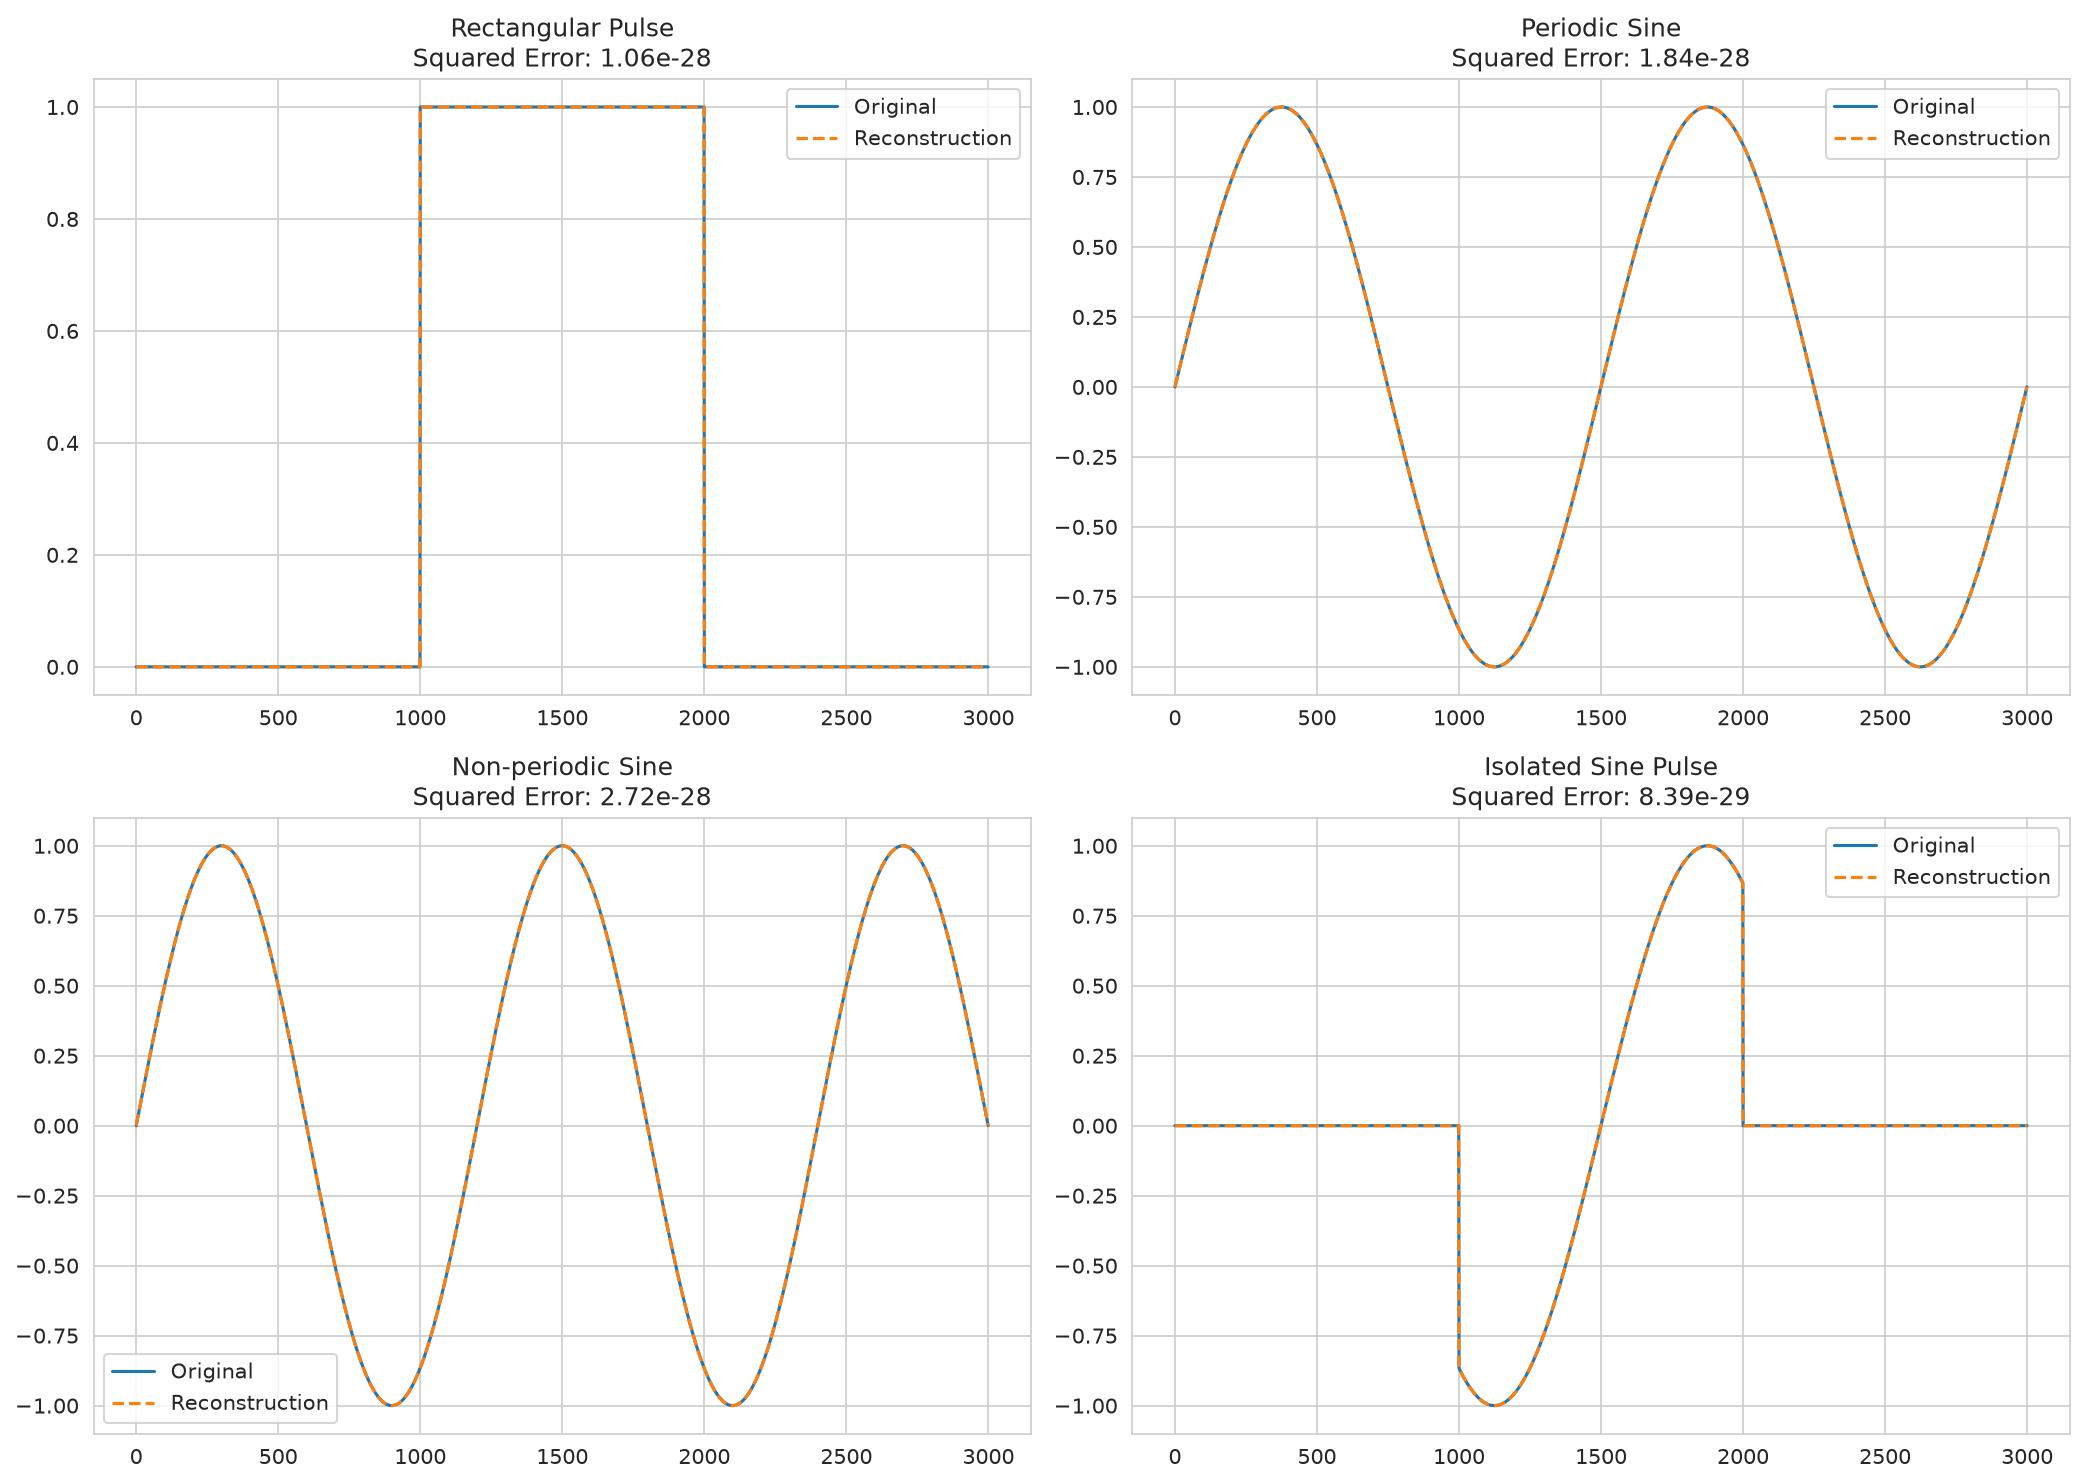
\includegraphics[width=\linewidth]{Images/signal_reconstruction.jpg}
\caption{Full-coefficient reconstruction of each synthetic signal; squared error at machine precision, confirming the FFT/iFFT pair is lossless.}
\label{fig:reconstruction}
\end{figure}

\begin{figure}[H]
\centering
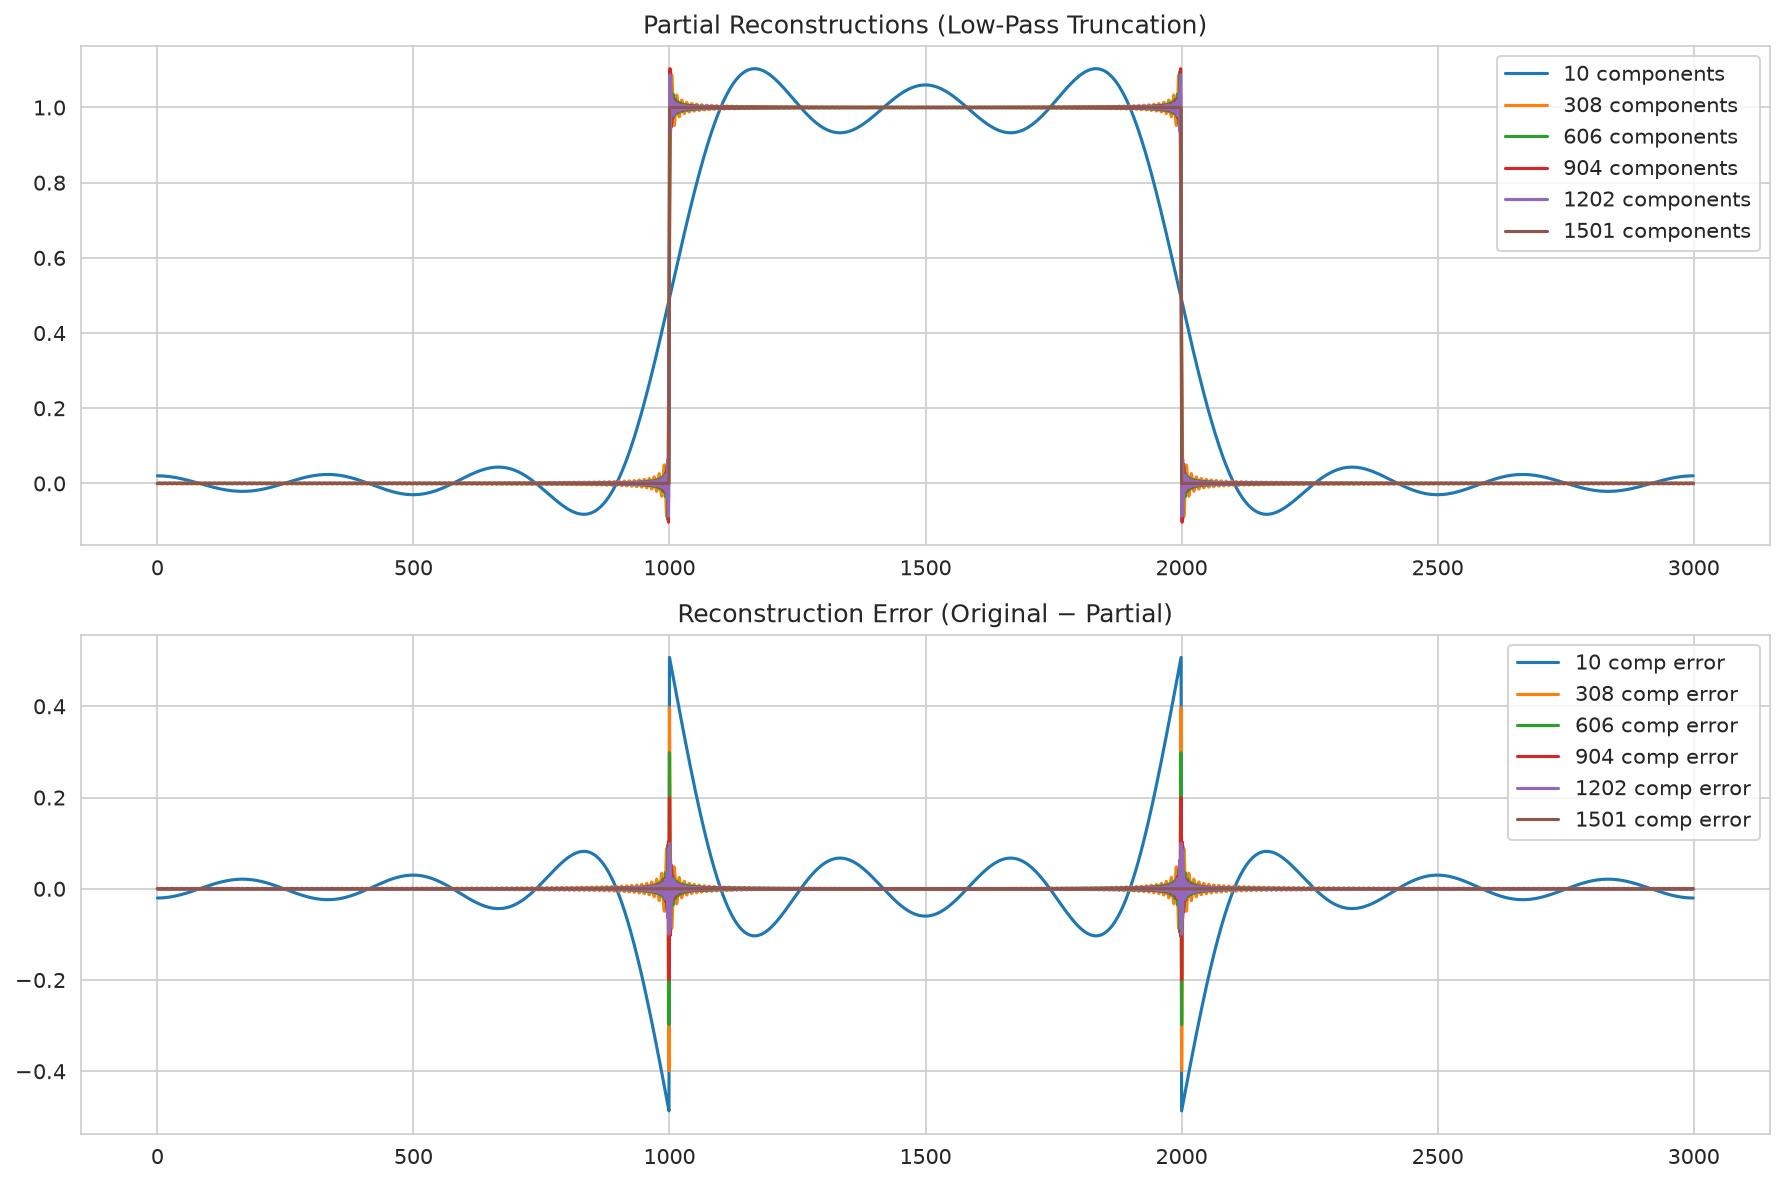
\includegraphics[width=\linewidth]{Images/partial_reconstruction.jpg}
\caption{Low-pass-truncated reconstructions of the rectangular pulse for increasing numbers of retained coefficients, and the reconstruction error.}
\label{fig:partialrecon}
\end{figure}

\begin{figure}[H]
\centering
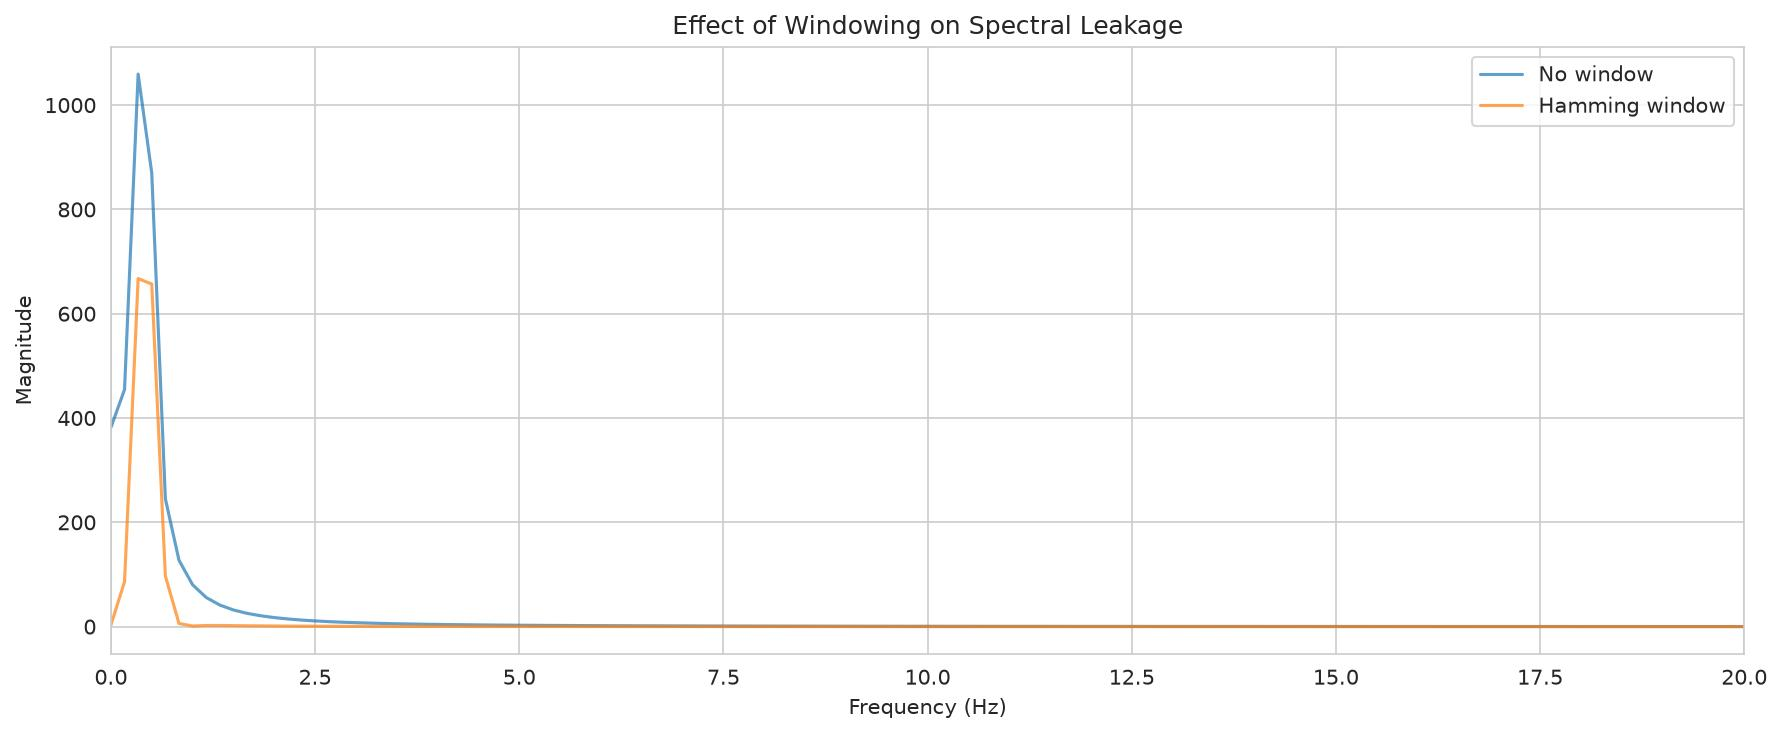
\includegraphics[width=\linewidth]{Images/windowing_effect.jpg}
\caption{Effect of a Hamming window on the non-periodic sine's spectrum: narrower main lobe, lower sidelobes -- reduced spectral leakage.}
\label{fig:windowing}
\end{figure}

\begin{figure}[H]
\centering
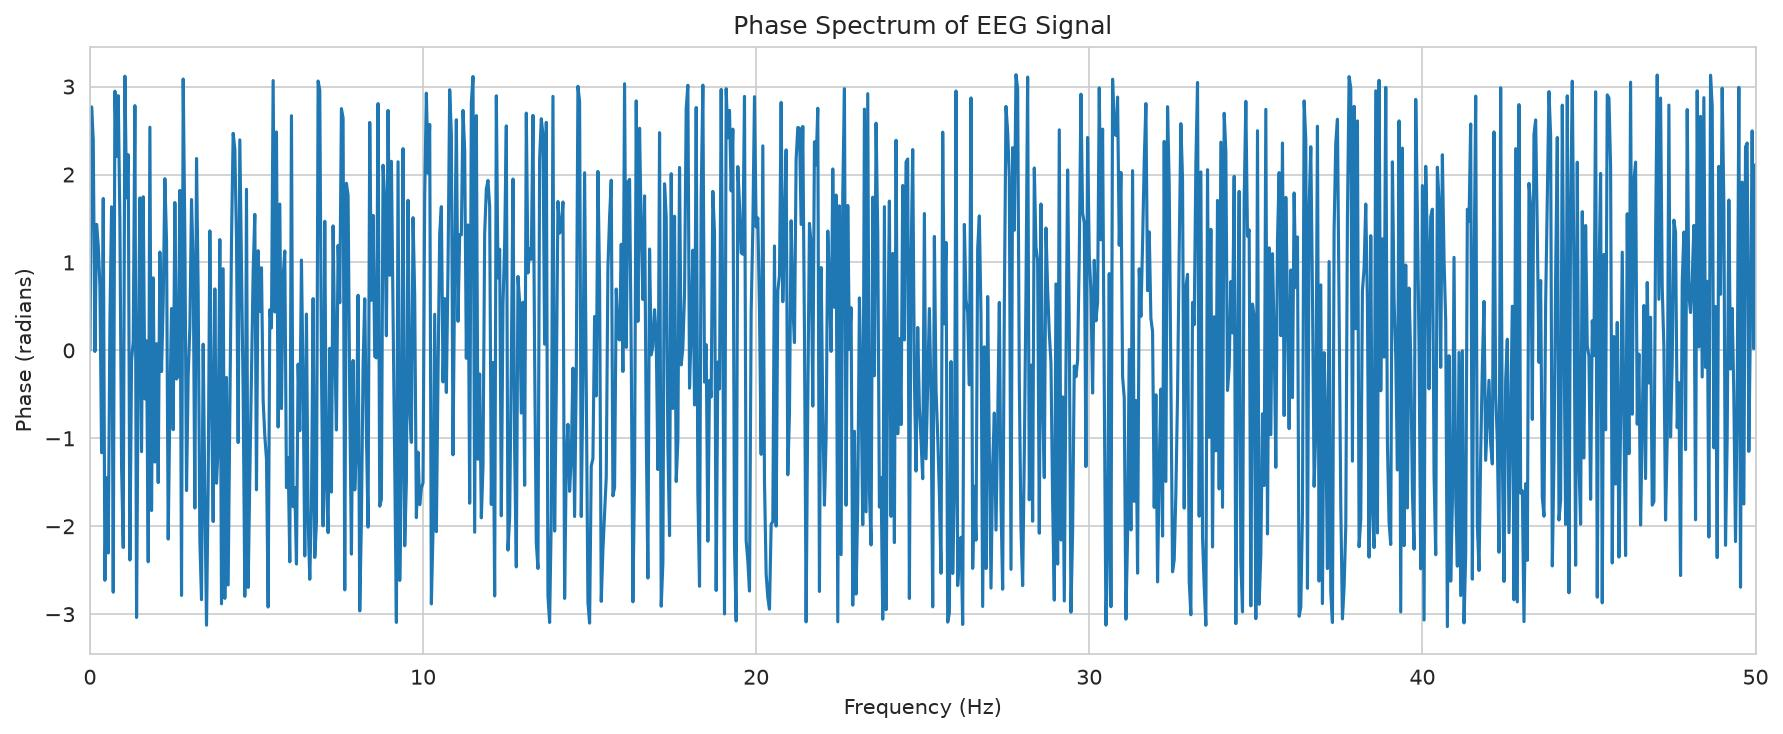
\includegraphics[width=\linewidth]{Images/phase_spectrum.jpg}
\caption{Phase spectrum of the EEG channel: effectively noise-like across frequency, as expected for a broadband physiological signal.}
\label{fig:phase}
\end{figure}

\begin{figure}[H]
\centering
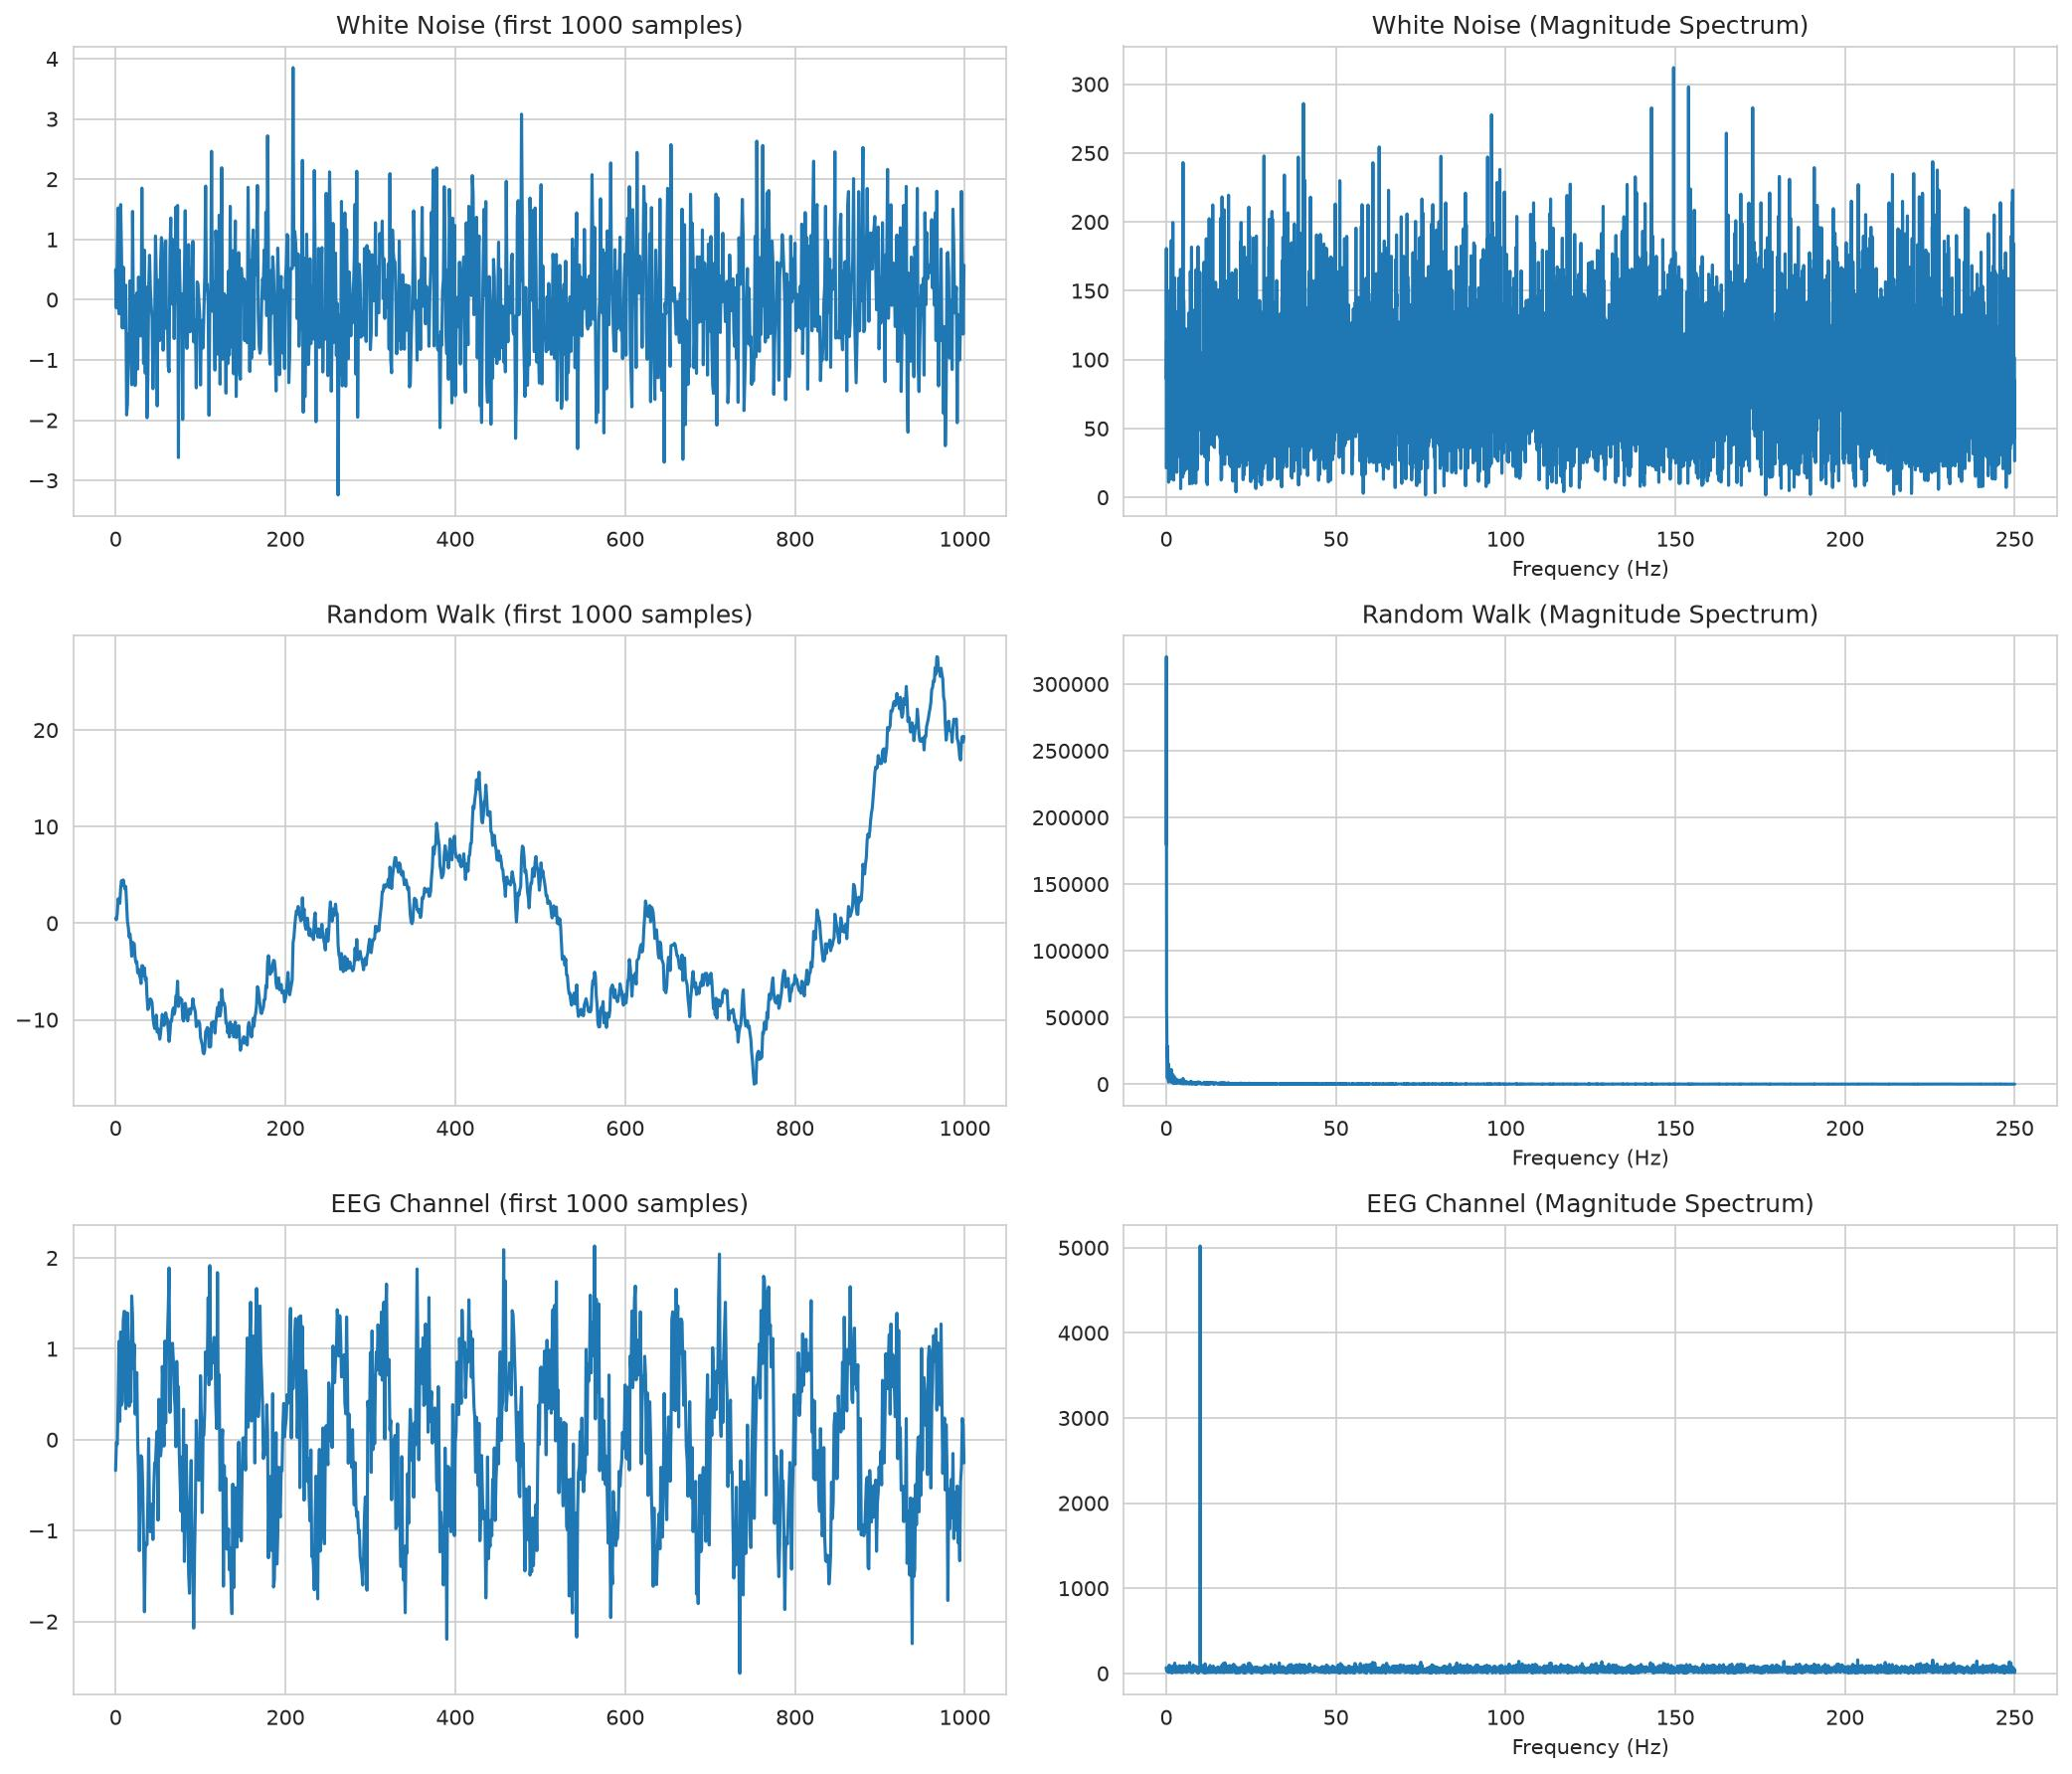
\includegraphics[width=\linewidth]{Images/real_signals_spectra.jpg}
\caption{First 1{,}000 samples and magnitude spectrum of white noise, a random walk, and the EEG channel (channel 8), computed identically for all three (Sec.~\ref{sec:spectral}).}
\label{fig:realspectra}
\end{figure}

\begin{figure}[H]
\centering
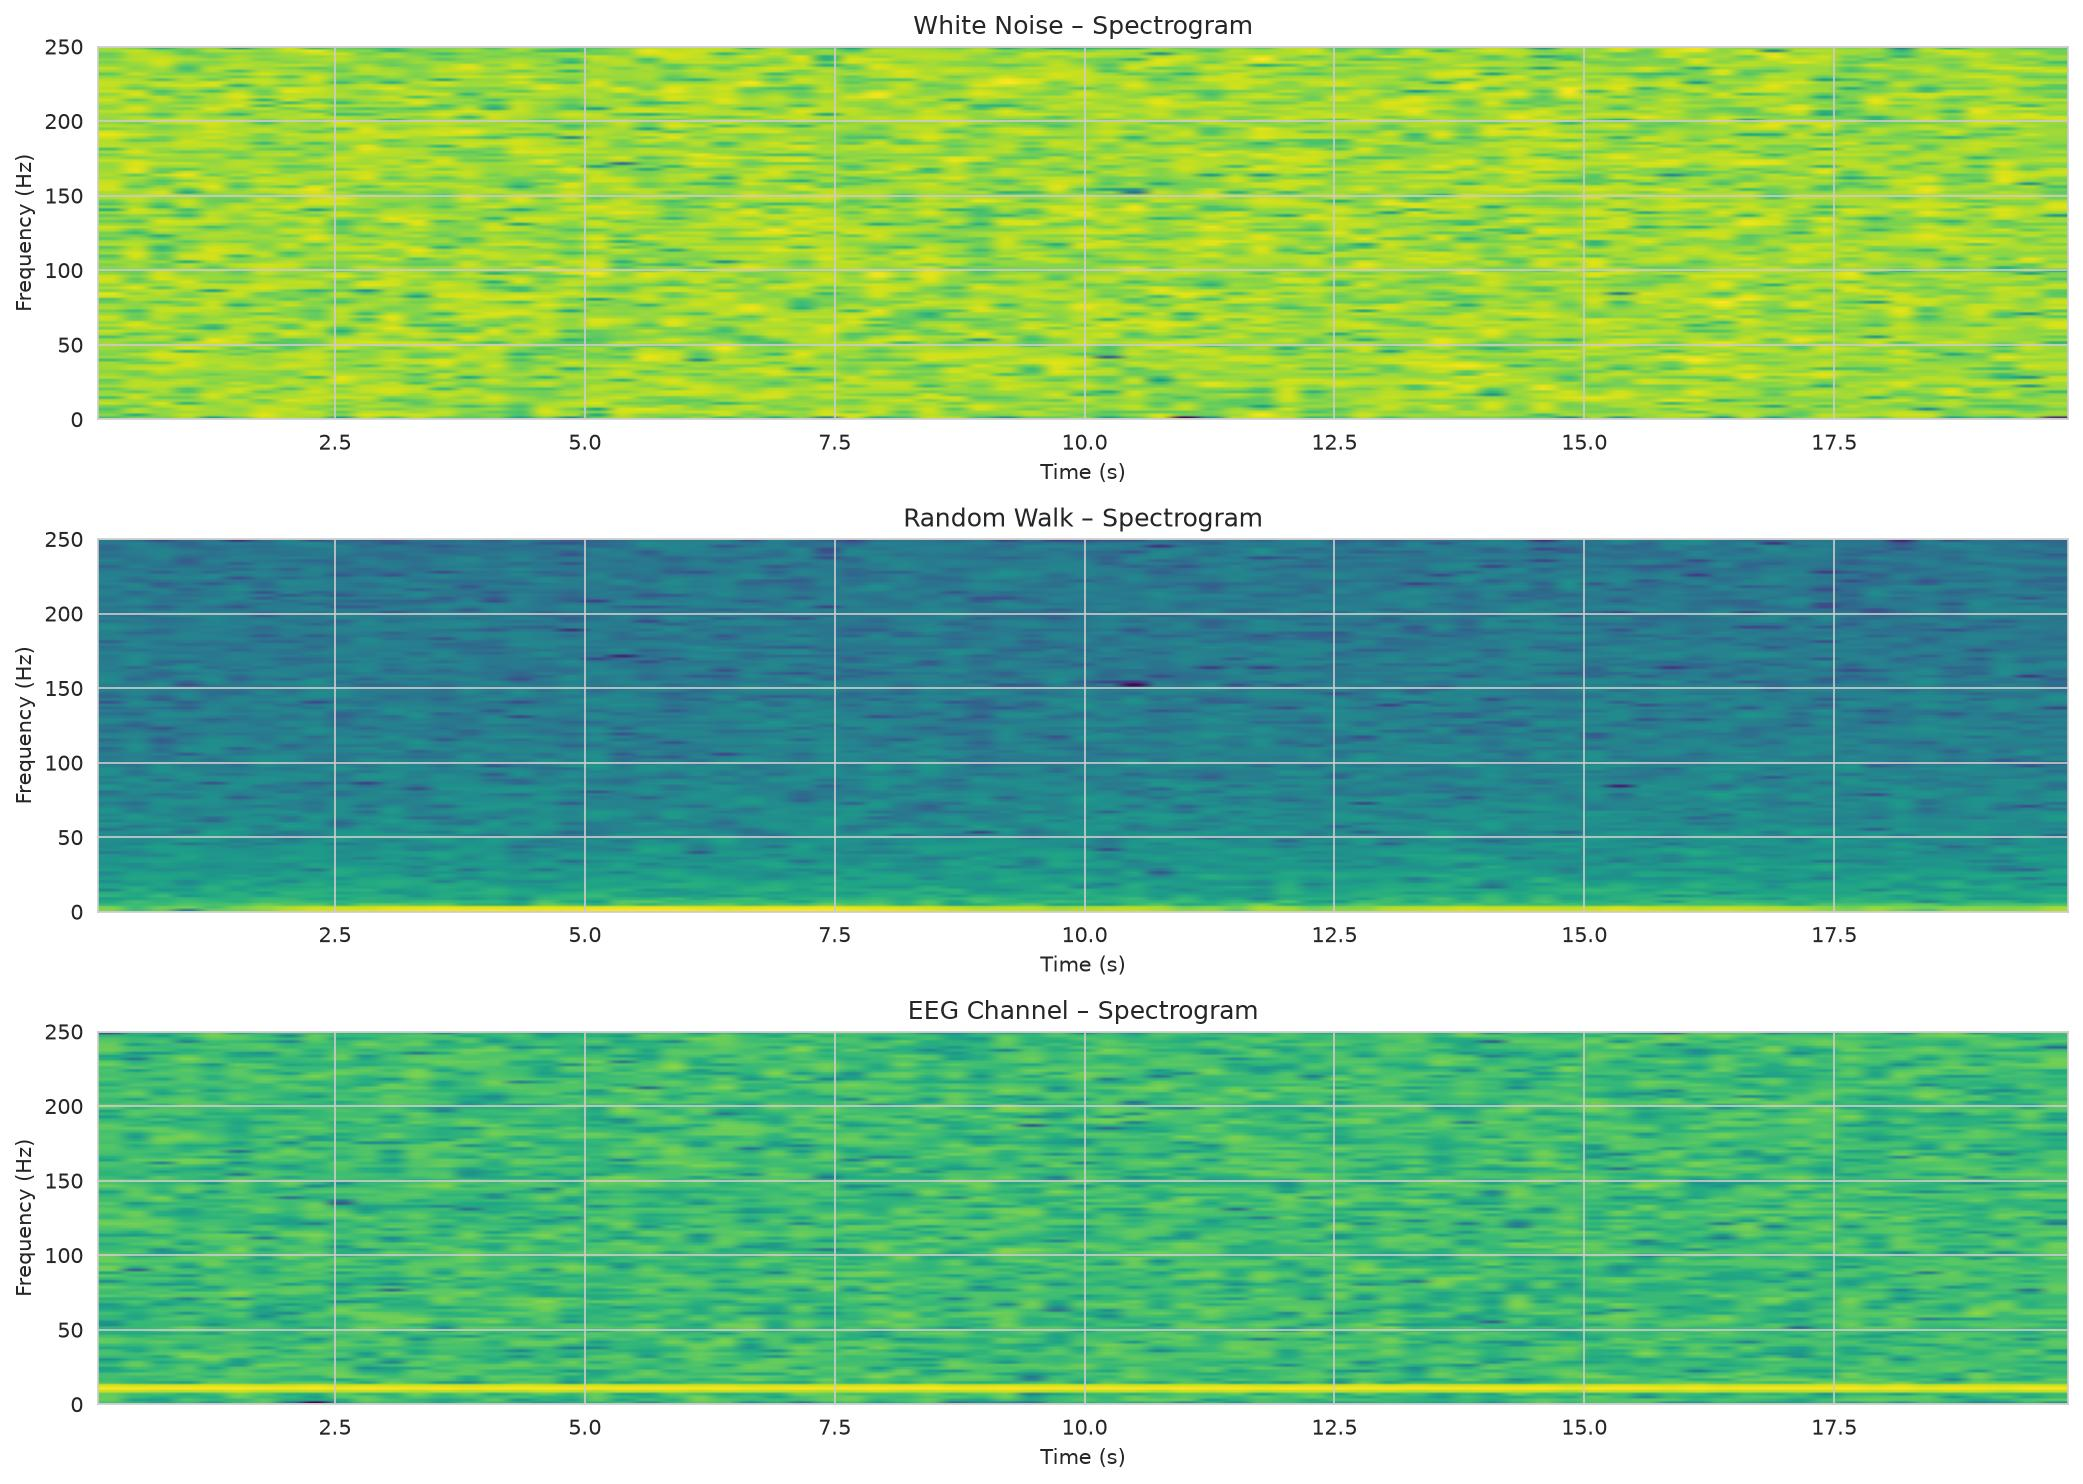
\includegraphics[width=\linewidth]{Images/spectrograms.jpg}
\caption{Spectrograms of white noise, random walk and the EEG channel: a persistent narrow-band component sits at $\approx$10~Hz (Alpha) throughout the recording.}
\label{fig:spectrograms}
\end{figure}

\begin{figure}[H]
\centering
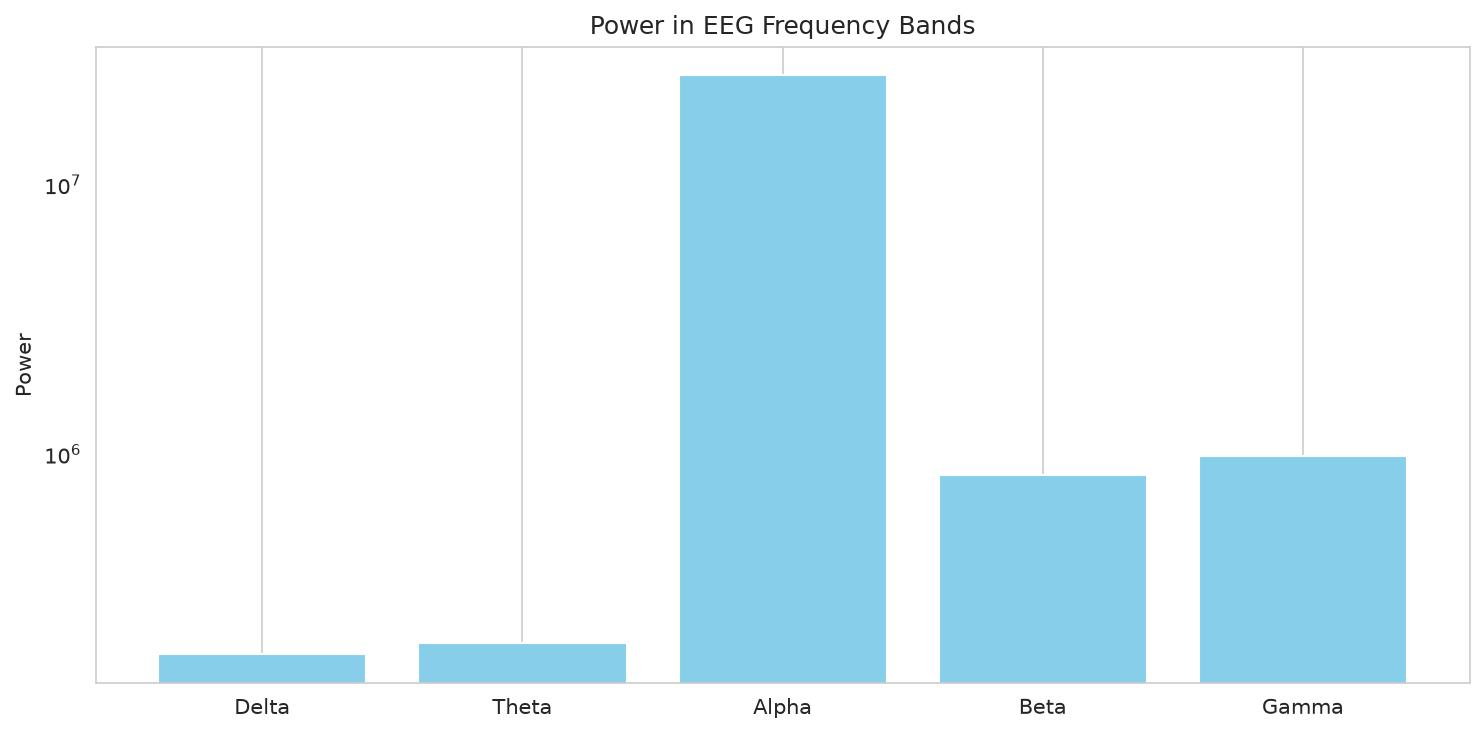
\includegraphics[width=\linewidth]{Images/band_power_bar.jpg}
\caption{Power in the five classical EEG bands (log scale), channel 8, first 10{,}000 samples, unfiltered.}
\label{fig:bandbar}
\end{figure}

\end{document}